%=== Préambule ===========================================================

\documentclass{beamer}
\usepackage{pdfpages}
\usepackage[english]{babel}
\usepackage{xspace}
\usepackage{pifont}
\usepackage{hyperref}
\usepackage{listings}
\usepackage{csquotes}
\usepackage{graphicx}
\usepackage{animate,media9} %,movie15}
\usepackage{wrapfig}
\usepackage{pdfpages}
\usepackage{tikz}
\usepackage{natbib}
\uselanguage{English}
\usepackage{fontawesome5}
\languagepath{English}
\setcounter{tocdepth}{1}
\usepackage{setspace}
\usepackage{amsmath}
\def\glasses{{\sffamily 
\leavevmode\rlap{%
\rotatebox[origin=tr]{125}{J}\kern1ex%  
\rotatebox[origin=tr]{125}{J}}% 
\rotatebox[origin=c]{-90}{D}%   
\rotatebox[origin=c]{-90}{D}}%
\def\ialy{\sffamily 
\resizebox{1ex}{1.5ex}{\reflectbox{\rotatebox[origin=]{75}{J}}}\kern-1pt%
\rlap{\tiny$\ ^\bullet\kern2.5pt^\bullet$ }%
\rotatebox[origin=c]{-90}{D}%   
\rotatebox[origin=c]{-90}{D}\kern-1pt%  
\resizebox{1ex}{1.5ex}{\rotatebox[origin=]{75}{J}}}}


\lstset{
  numbers=left,
  basicstyle=\tiny\ttfamily,      
  breaklines=true, 
  showtabs=false,
  showstringspaces=false,
}  

%=== Configuration de Beamer et du thème metropolis ======================
\usepackage{bbding}
\usetheme[background=light]{metropolis}
\usepackage[clock]{ifsym}

\definecolor{mLightBrown}{HTML}{000000}
\definecolor{black}{HTML}{000000}
\setbeamercolor{structure}{fg=black,bg=mLightBrown}
\setbeamercolor{palette primary}{%
	use=normal text,
	fg=normal text.bg,
	bg=mLightBrown
}
%\setsansfont[BoldFont={Linux Libertine G Bold},Numbers={OldStyle}]{Linux Libertine G}

\metroset{block=fill}

%=== Page de titre =======================================================

%path to logo and biblio -> to be adapted to your local directories 
\newcommand\dirlogo{../../logos/}
\newcommand\dirbiblio{../../biblio/}



\title{{\normalsize \vskip 1cm Exploring complex normal faulting systems through physics-based dynamic rupture modeling}}
\subtitle{\small 5 min talk !}
\author{Hugo S. \\ {\tiny Institut de Recherche pour le Développement IRD - ISTerre} \\ 
O., Scotti, S., Hok, A.-A. Gabriel and T. Taufiqurrahman \\
\\
\textit{ANR EQTIME Project}
}

\date[2021]{\today}

\subject{Group Meeting}

\titlegraphic{\centering \vspace{-15pt}
\includegraphics[height=1.3cm]{../../logos/logo_all_presentation.pdf} \par} %\qquad  
\includegraphics[height=1.4cm]{../../logos/anr_eqtime.png} \par }


\addtobeamertemplate{frametitle}{}{%
\begin{tikzpicture}[remember picture,overlay]
  \node[anchor=north east,yshift=0.0ex] at (current page.north east) {
\includegraphics[height=4ex]{../../logos/logo_irsn}};
  %\node[anchor=north east,yshift=0.5ex] at (current page.north east) {\includegraphics[height=3.3ex]{\dirlogo/seiscope_color_light_background}};
\end{tikzpicture}}



%=== Document ============================================================

\begin{document}

% --- Préambule ---------------------------------------------------------------

\begin{frame}
    \titlepage
\end{frame}

\begin{frame}
 {Outline}
 
 \tableofcontents
 
\end{frame}


\begin{frame}
 {Who am I?}
 
 Hugo S. S\'anchez-Reyes : \\
 \vskip 1cm
 \begin{minipage}{1\linewidth}
    \begin{itemize}
        \item \scriptsize 2019 -- PhD. Earth Sciences, Universit\'e de Grenoble Alpes, France 
        \item \scriptsize 2020 -- Postdoc at Universit\'e Grenoble de Alpes, France
        \item \scriptsize 2021 -- Postdoc at the Institut de Radioprotection et S\^uret\'e Nucleaire (IRSN)
        \item \scriptsize 2022 -- Researcher at Institute of Research for Development (IRD, ISTerre)
        \vskip 0.8cm
        \item[\ding{43}] Ah, by the way ... {\bf I am visually impaired! \glasses }
    \end{itemize}  
 \end{minipage}

\end{frame}


\section{Motivation}


\begin{frame}
 {Seismic Hazard in Central Italy}
 
 \begin{center}
  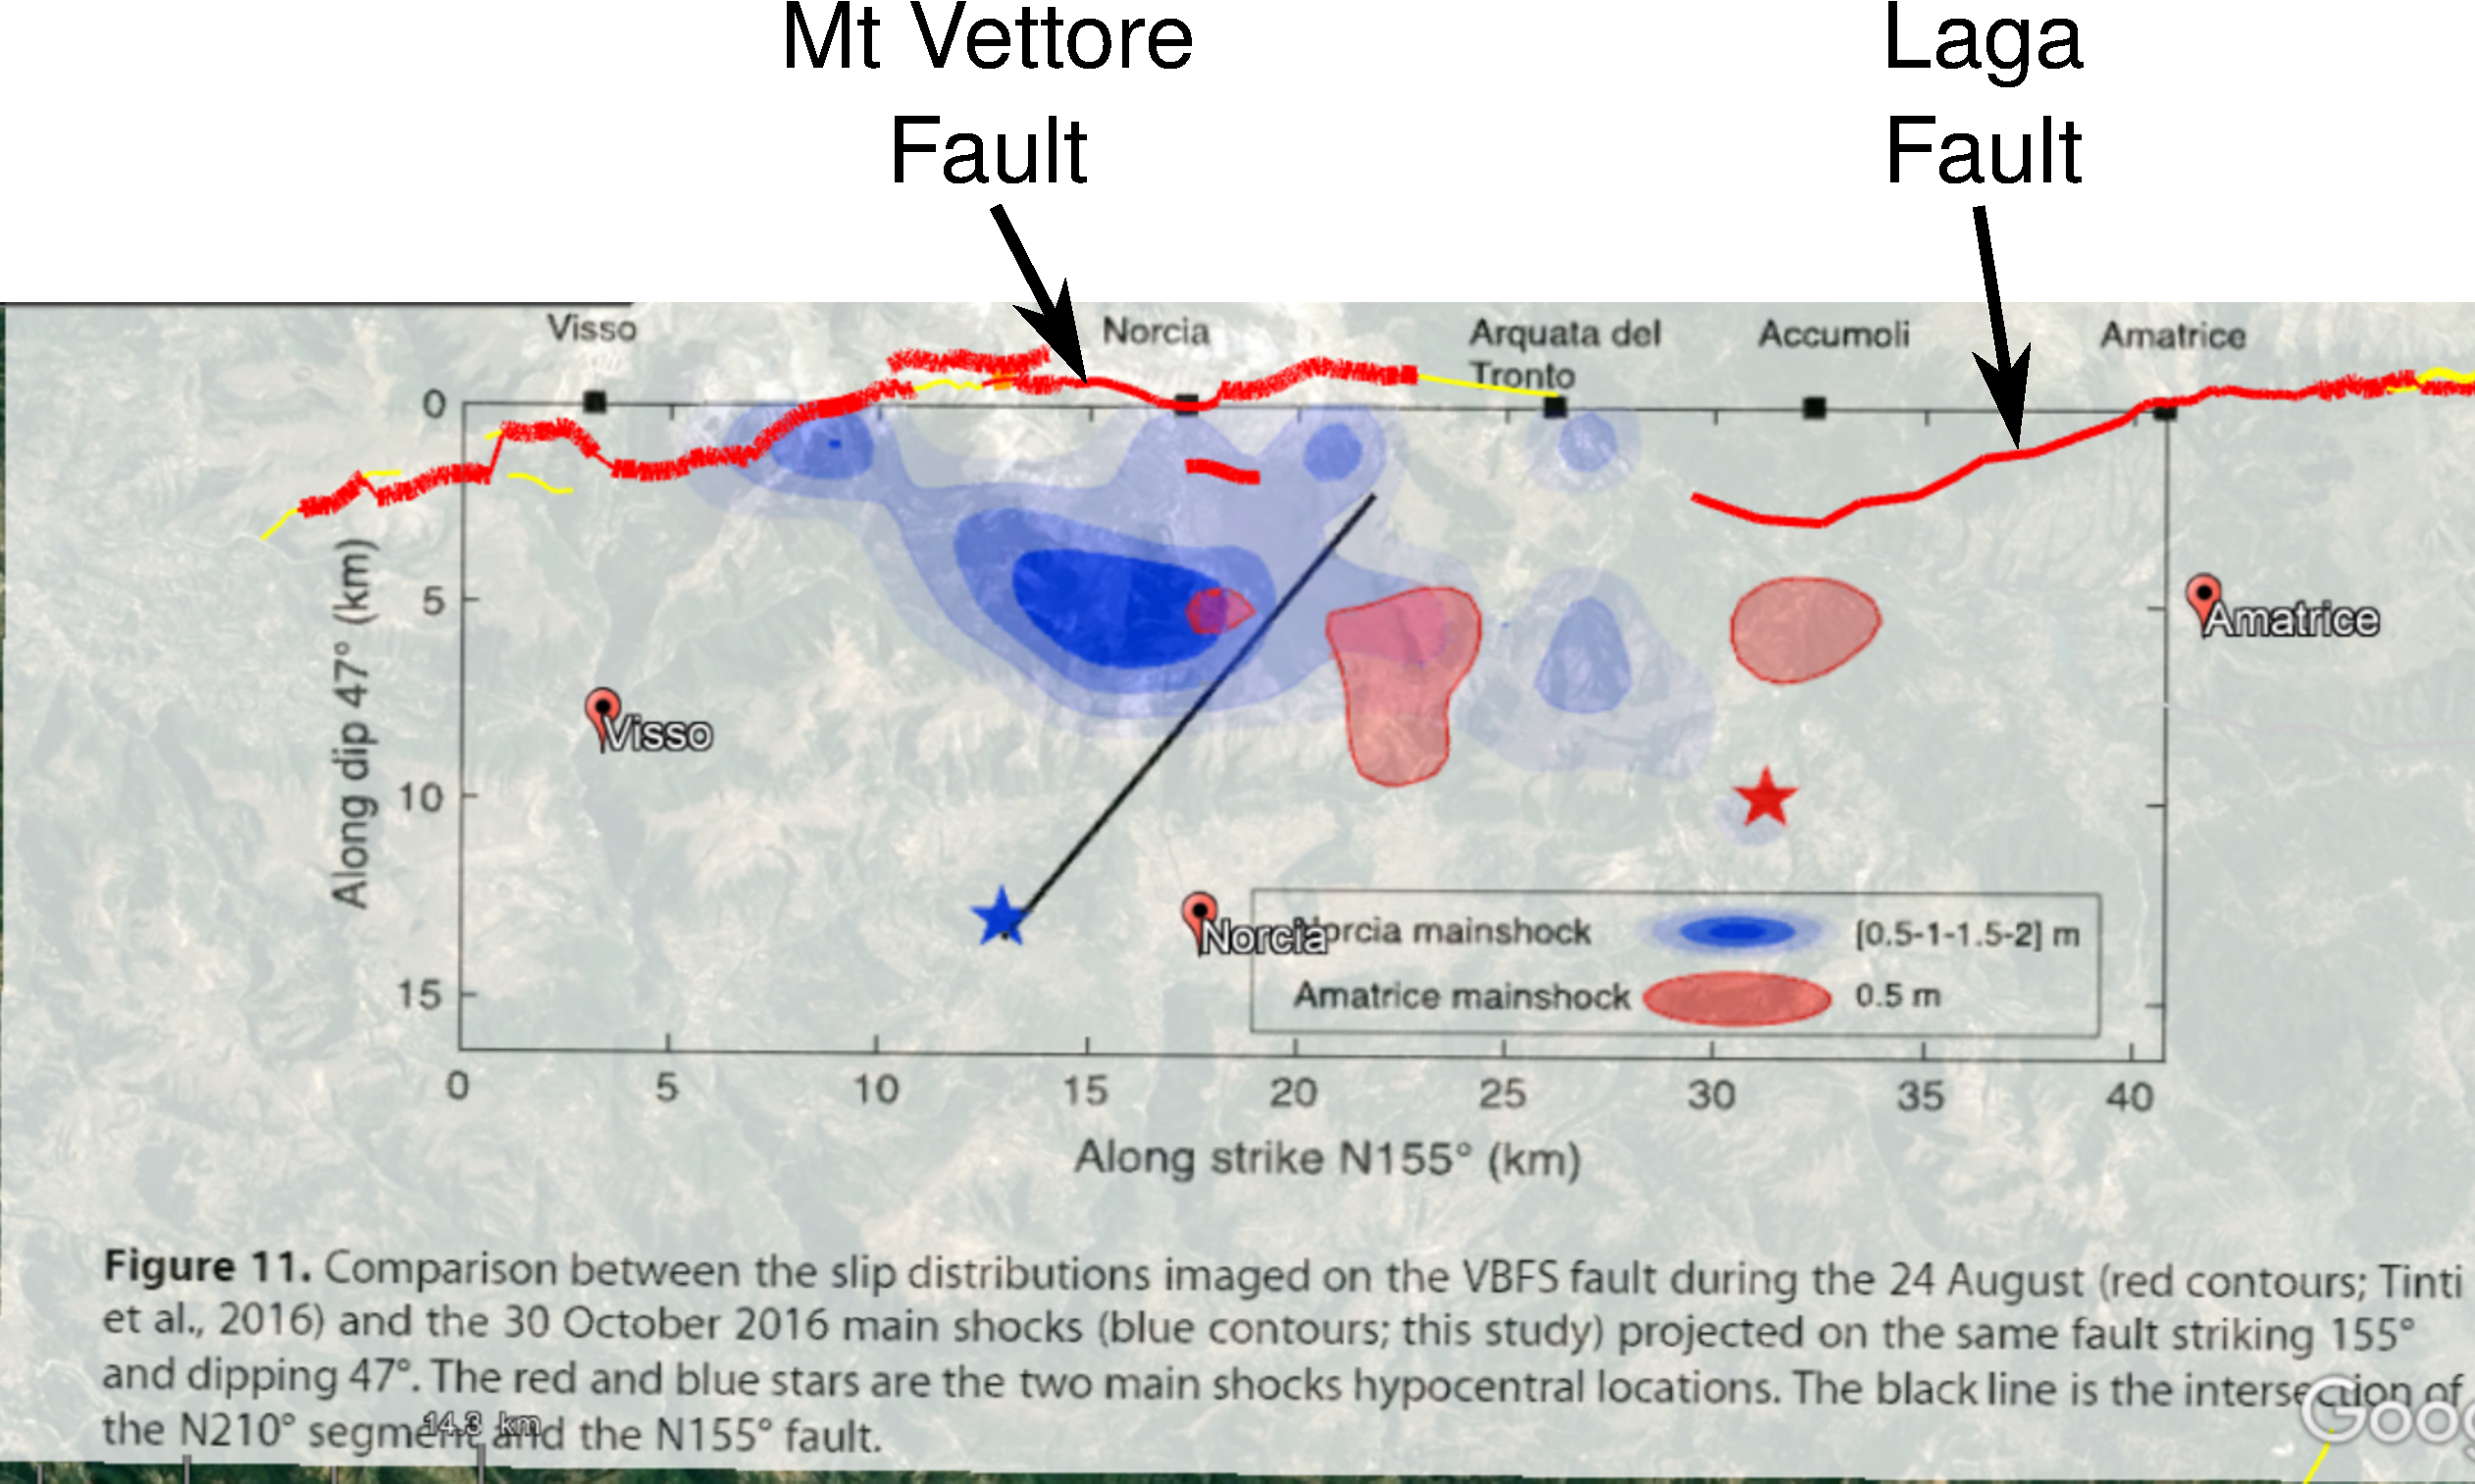
\includegraphics[width=0.65\linewidth]{images/amatrice_1.pdf} \,
  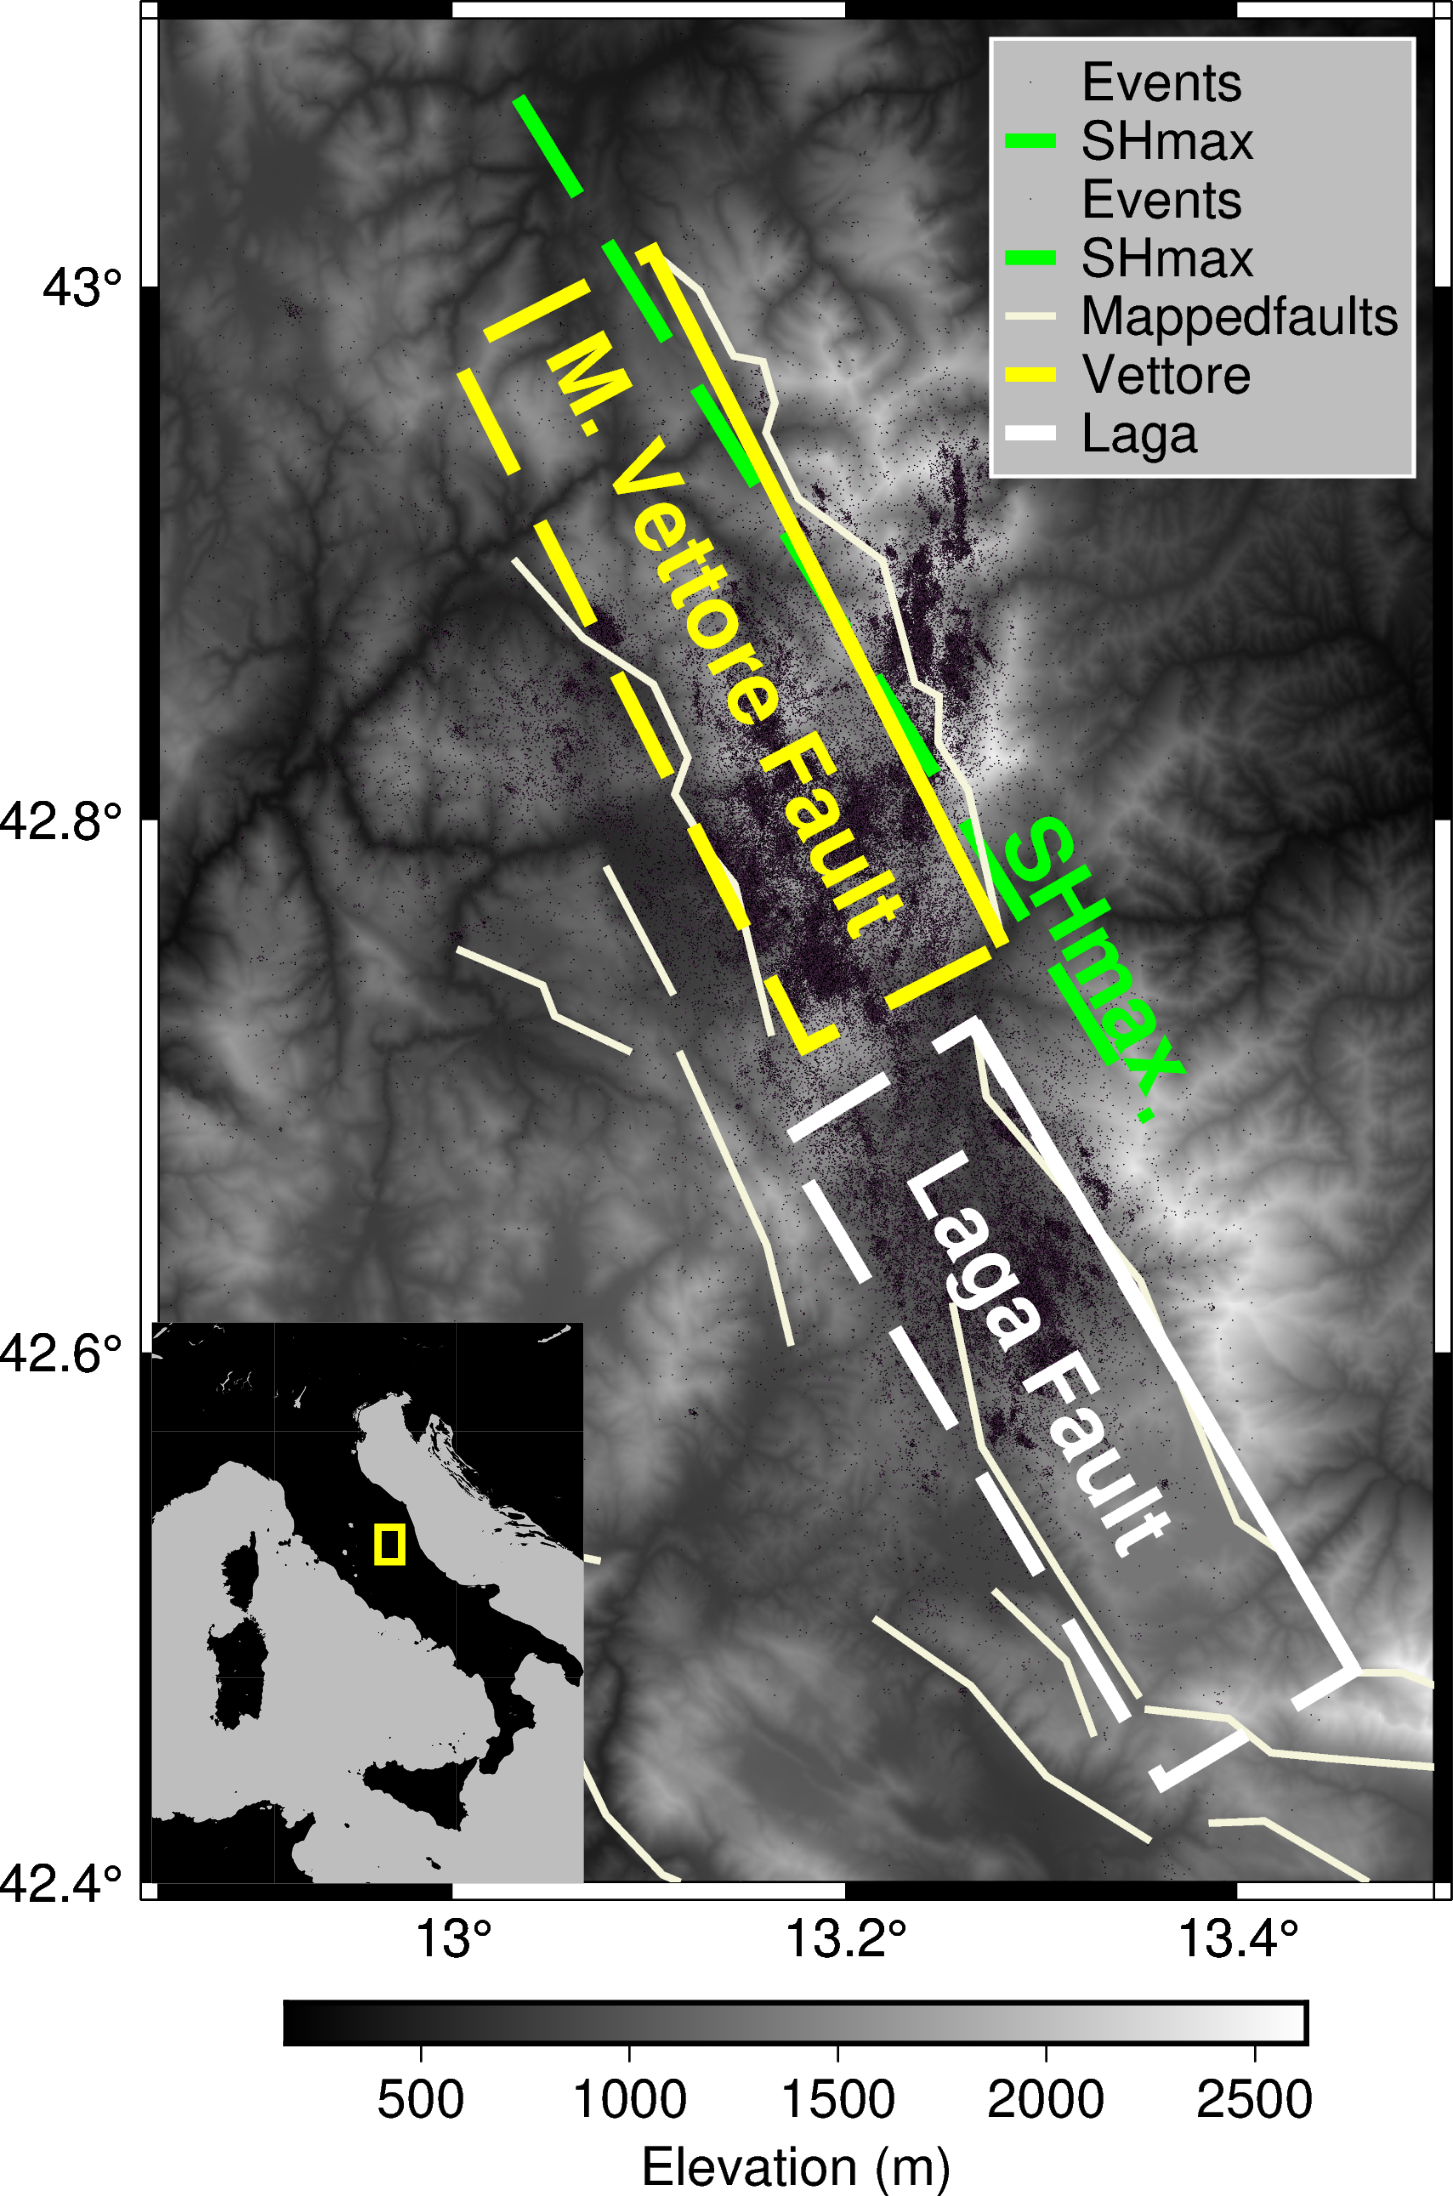
\includegraphics[width=0.3\linewidth]{images/map_italy.png}  
 \end{center}
  \vskip 0.2cm
  {\bf \hfill \scriptsize Modified by O. Scotti from \cite{Scognamiglio_2018_CFG}}
  
\end{frame}

\begin{frame}
 {Seismic Hazard in Central Italy}
 
 \begin{center}
    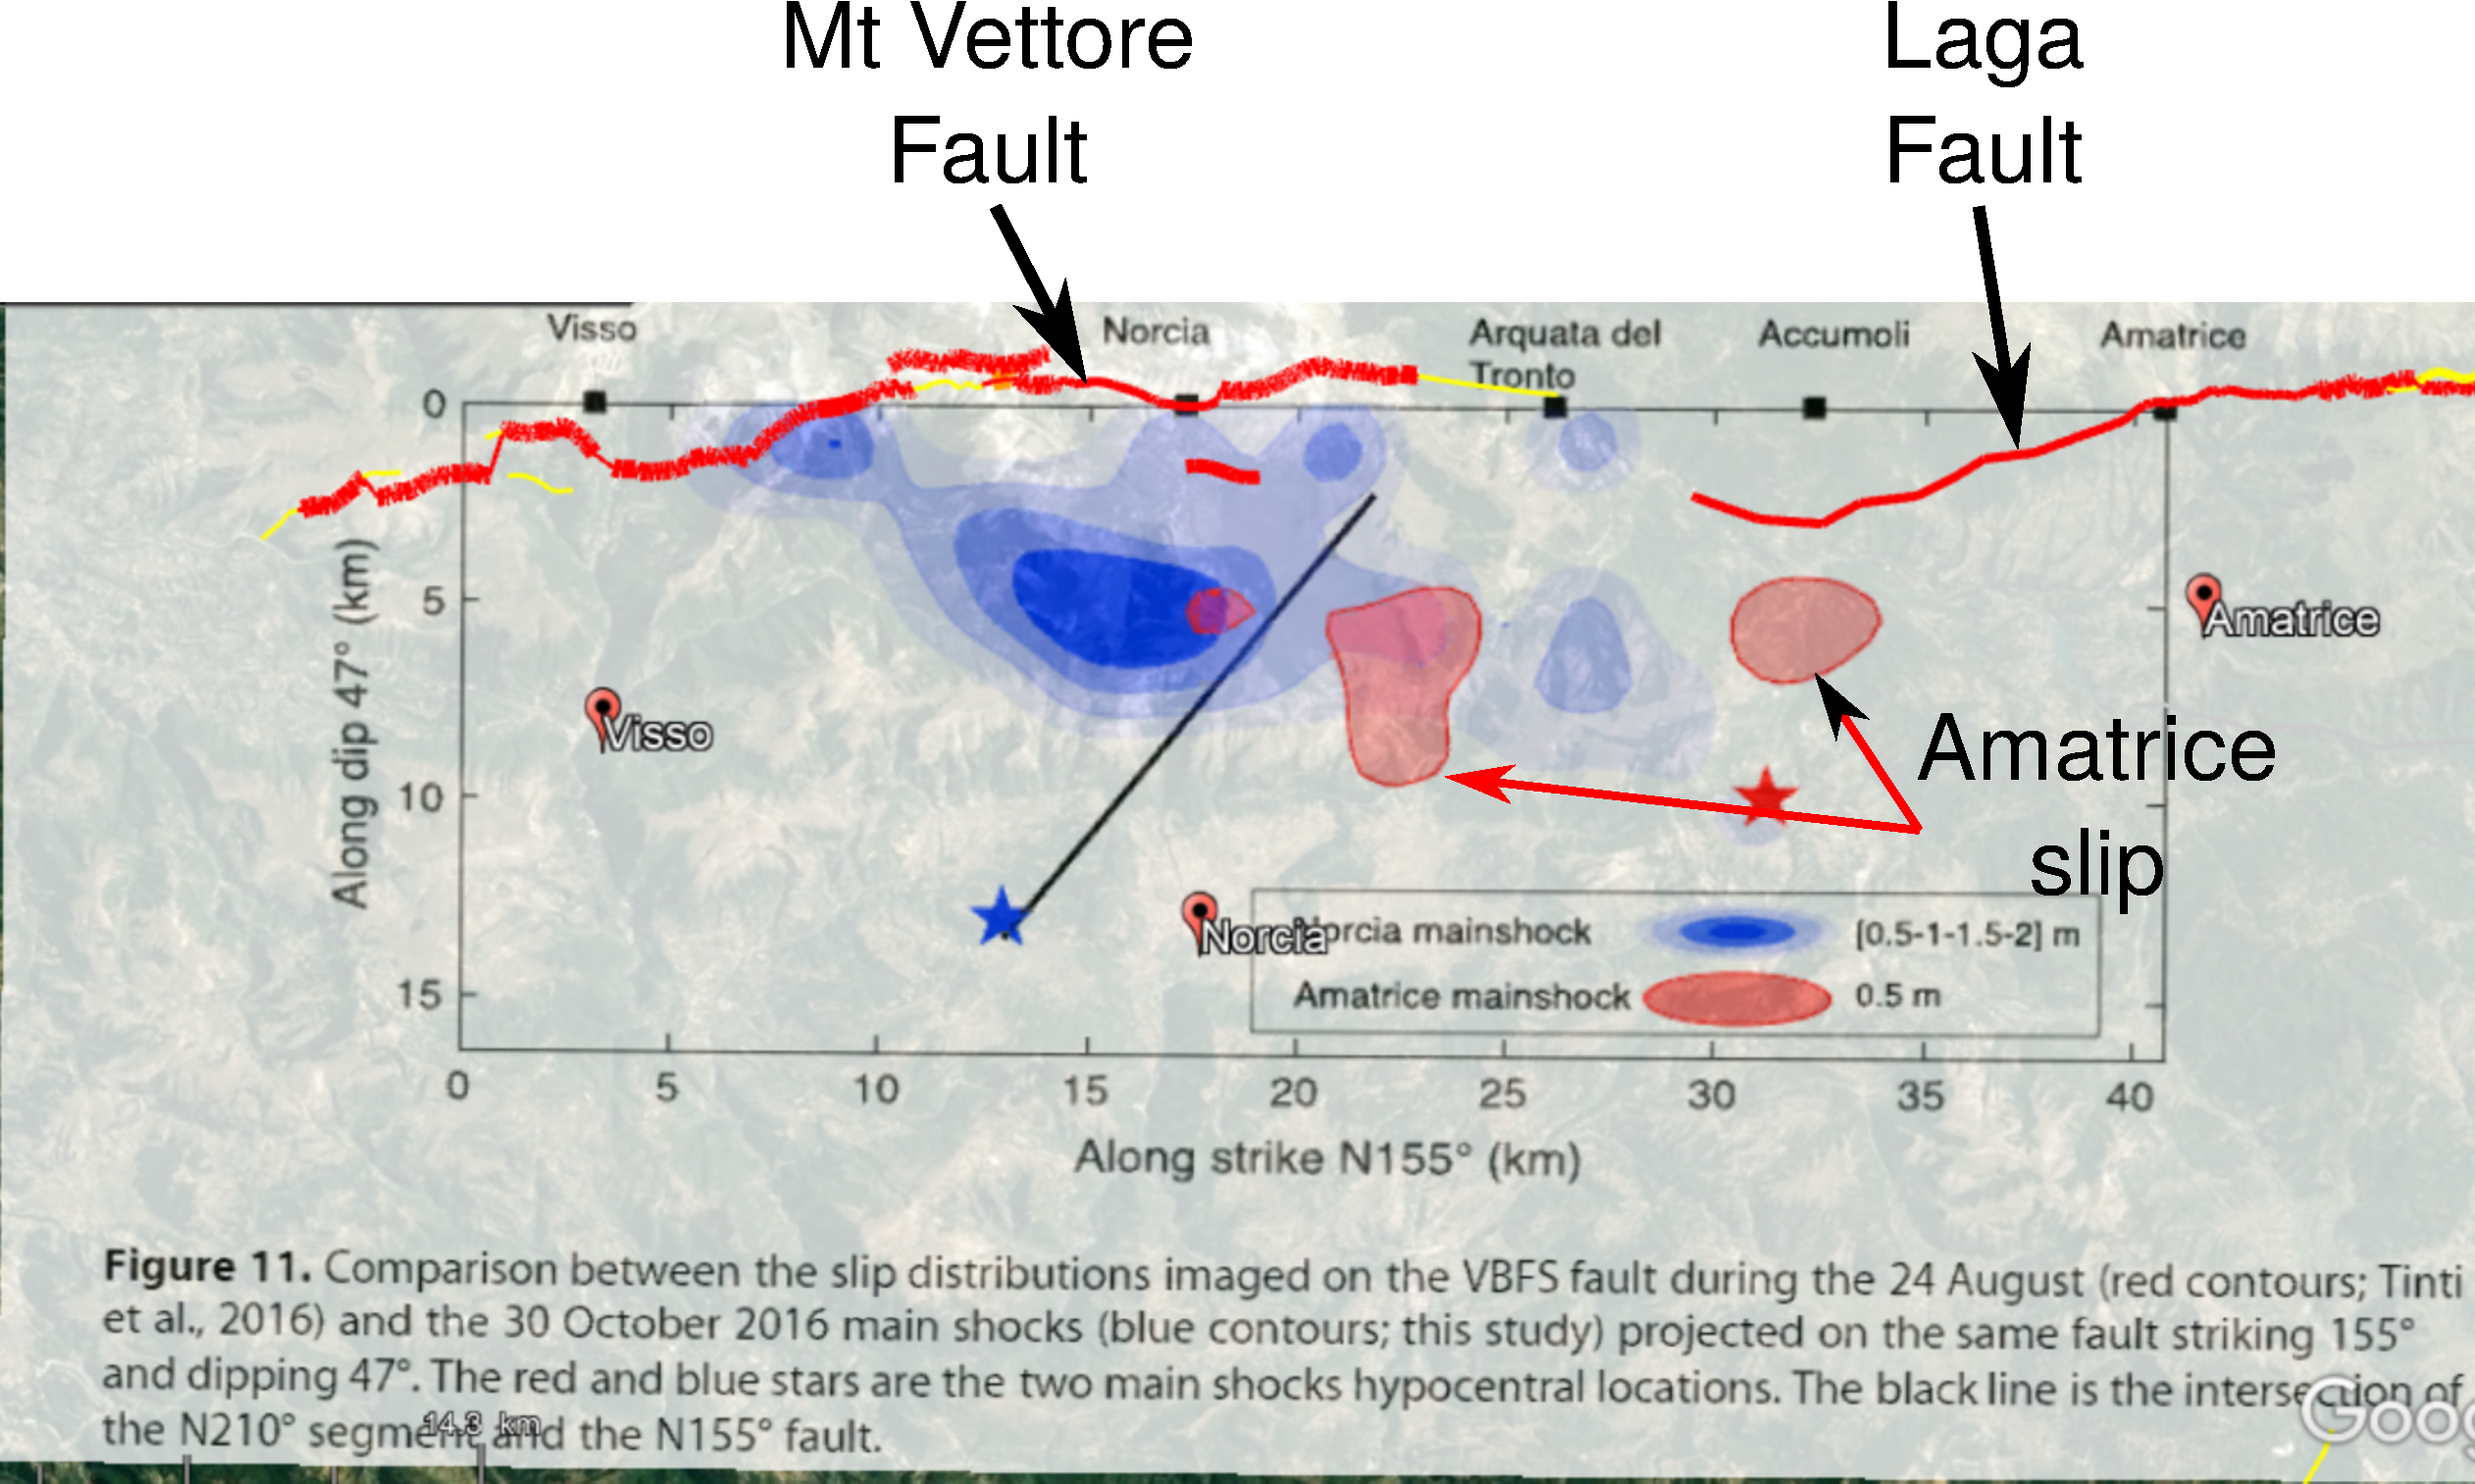
\includegraphics[width=0.65\linewidth]{images/amatrice_2.pdf} \,
    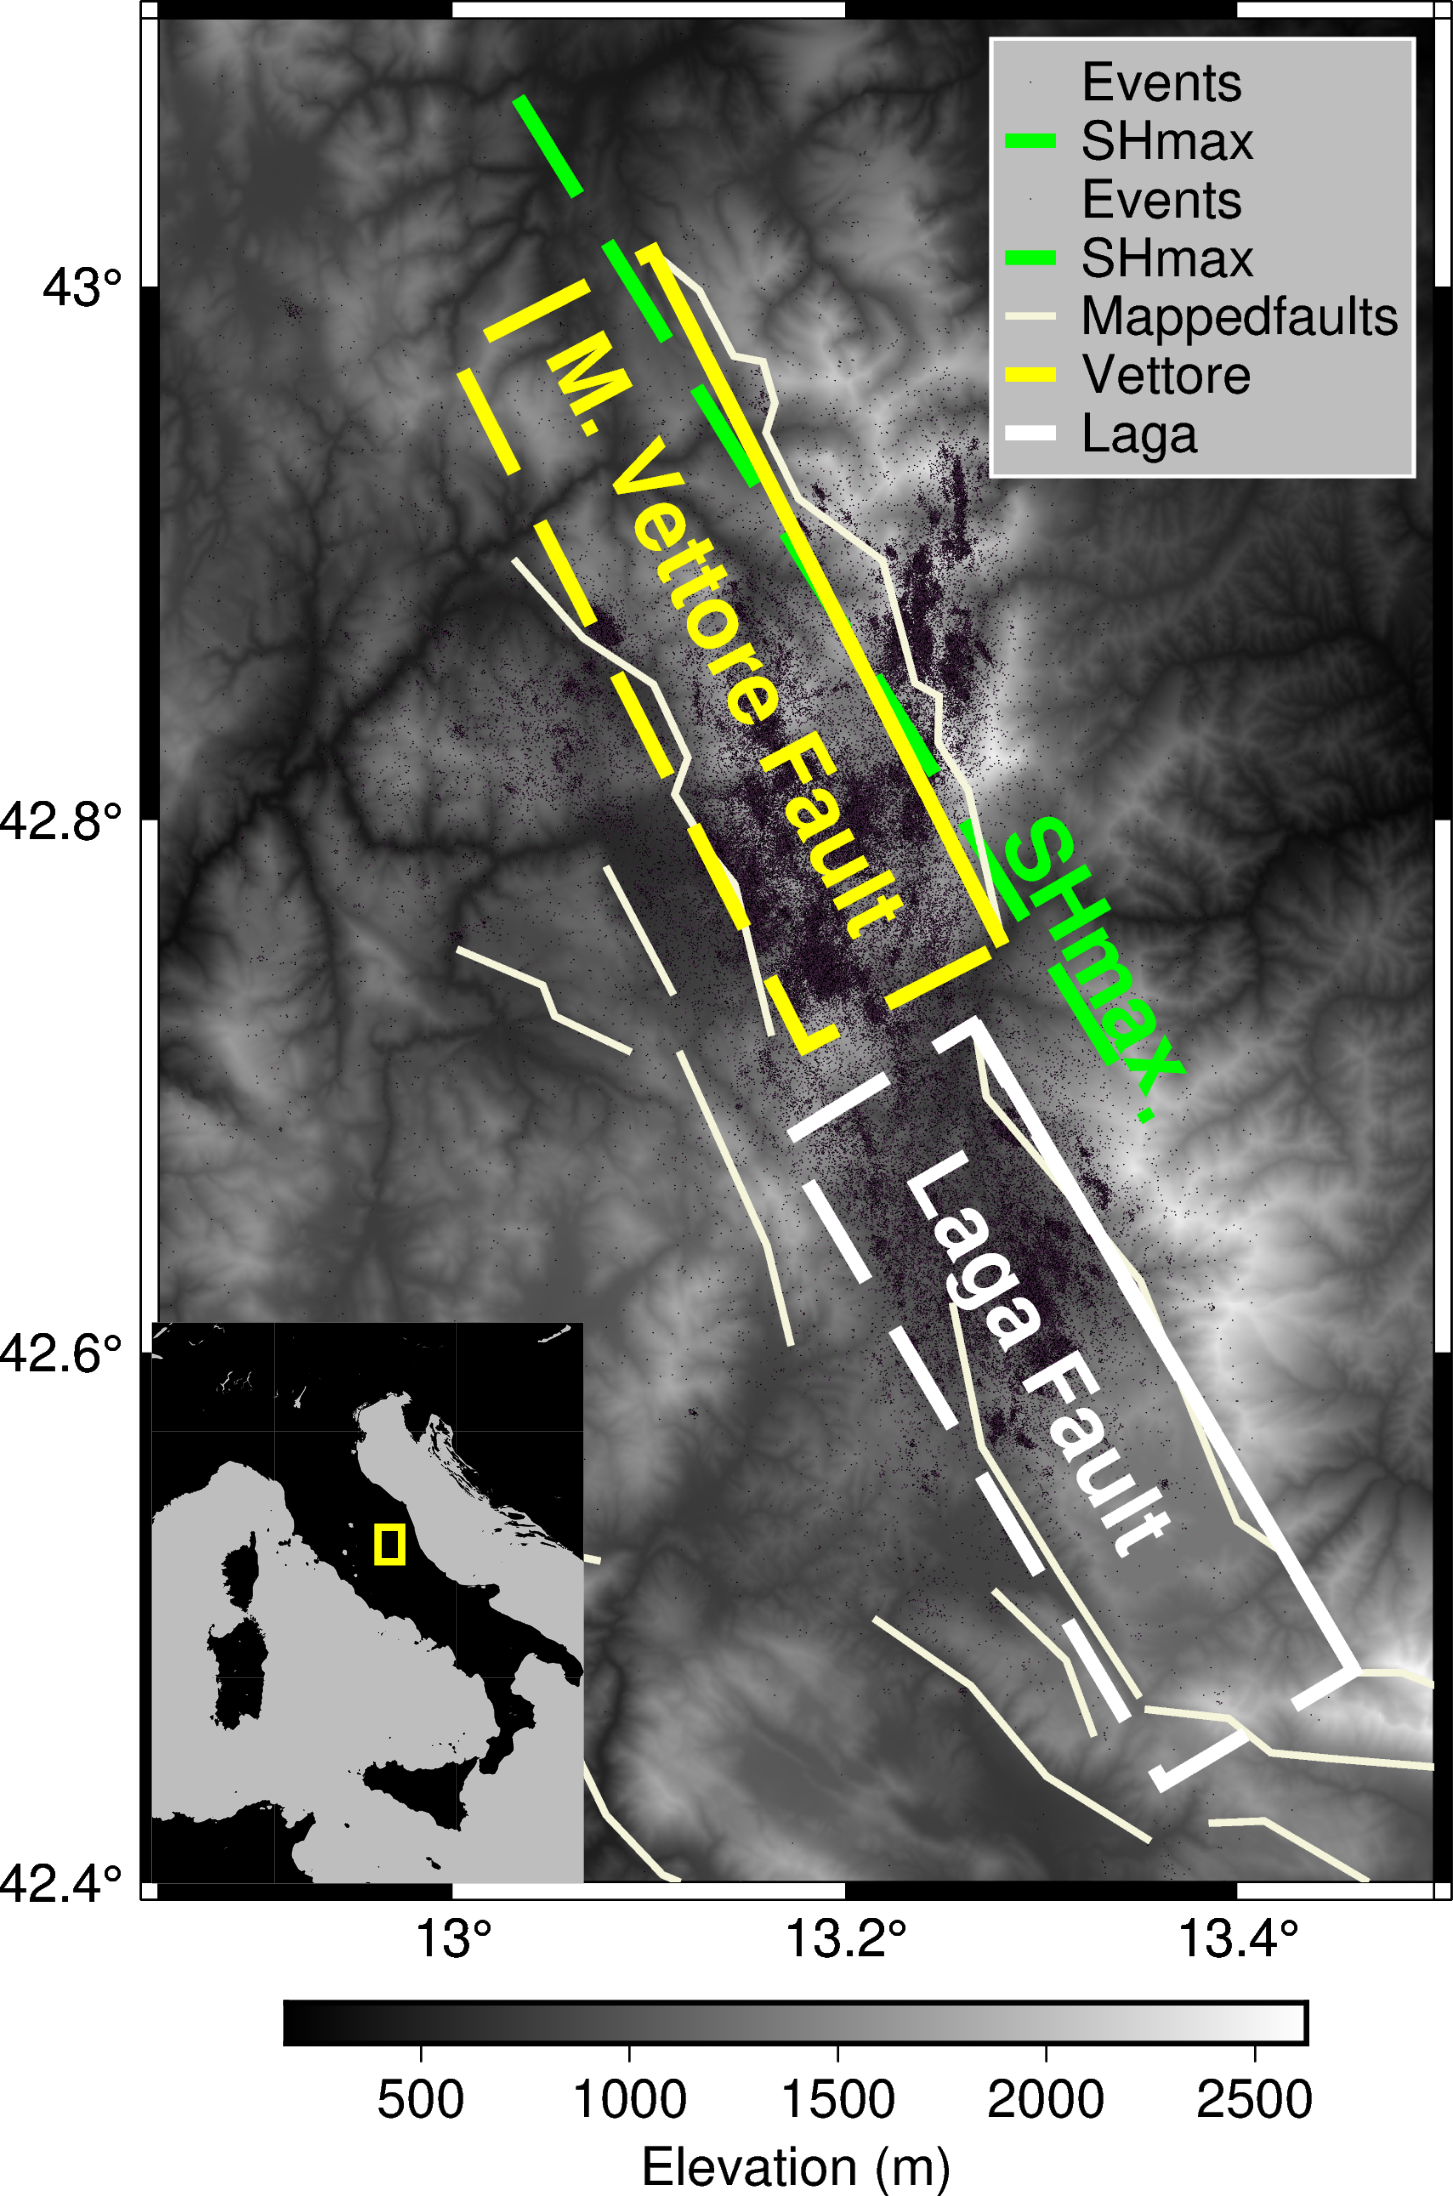
\includegraphics[width=0.3\linewidth]{images/map_italy.png}  
 \end{center}
  \vskip 0.2cm
  {\bf \hfill \scriptsize Modified by O. Scotti from \cite{Scognamiglio_2018_CFG}}
  \addtocounter{framenumber}{-1}
  
\end{frame}


\begin{frame}
 {Seismic Hazard in Central Italy}

 \begin{center}
  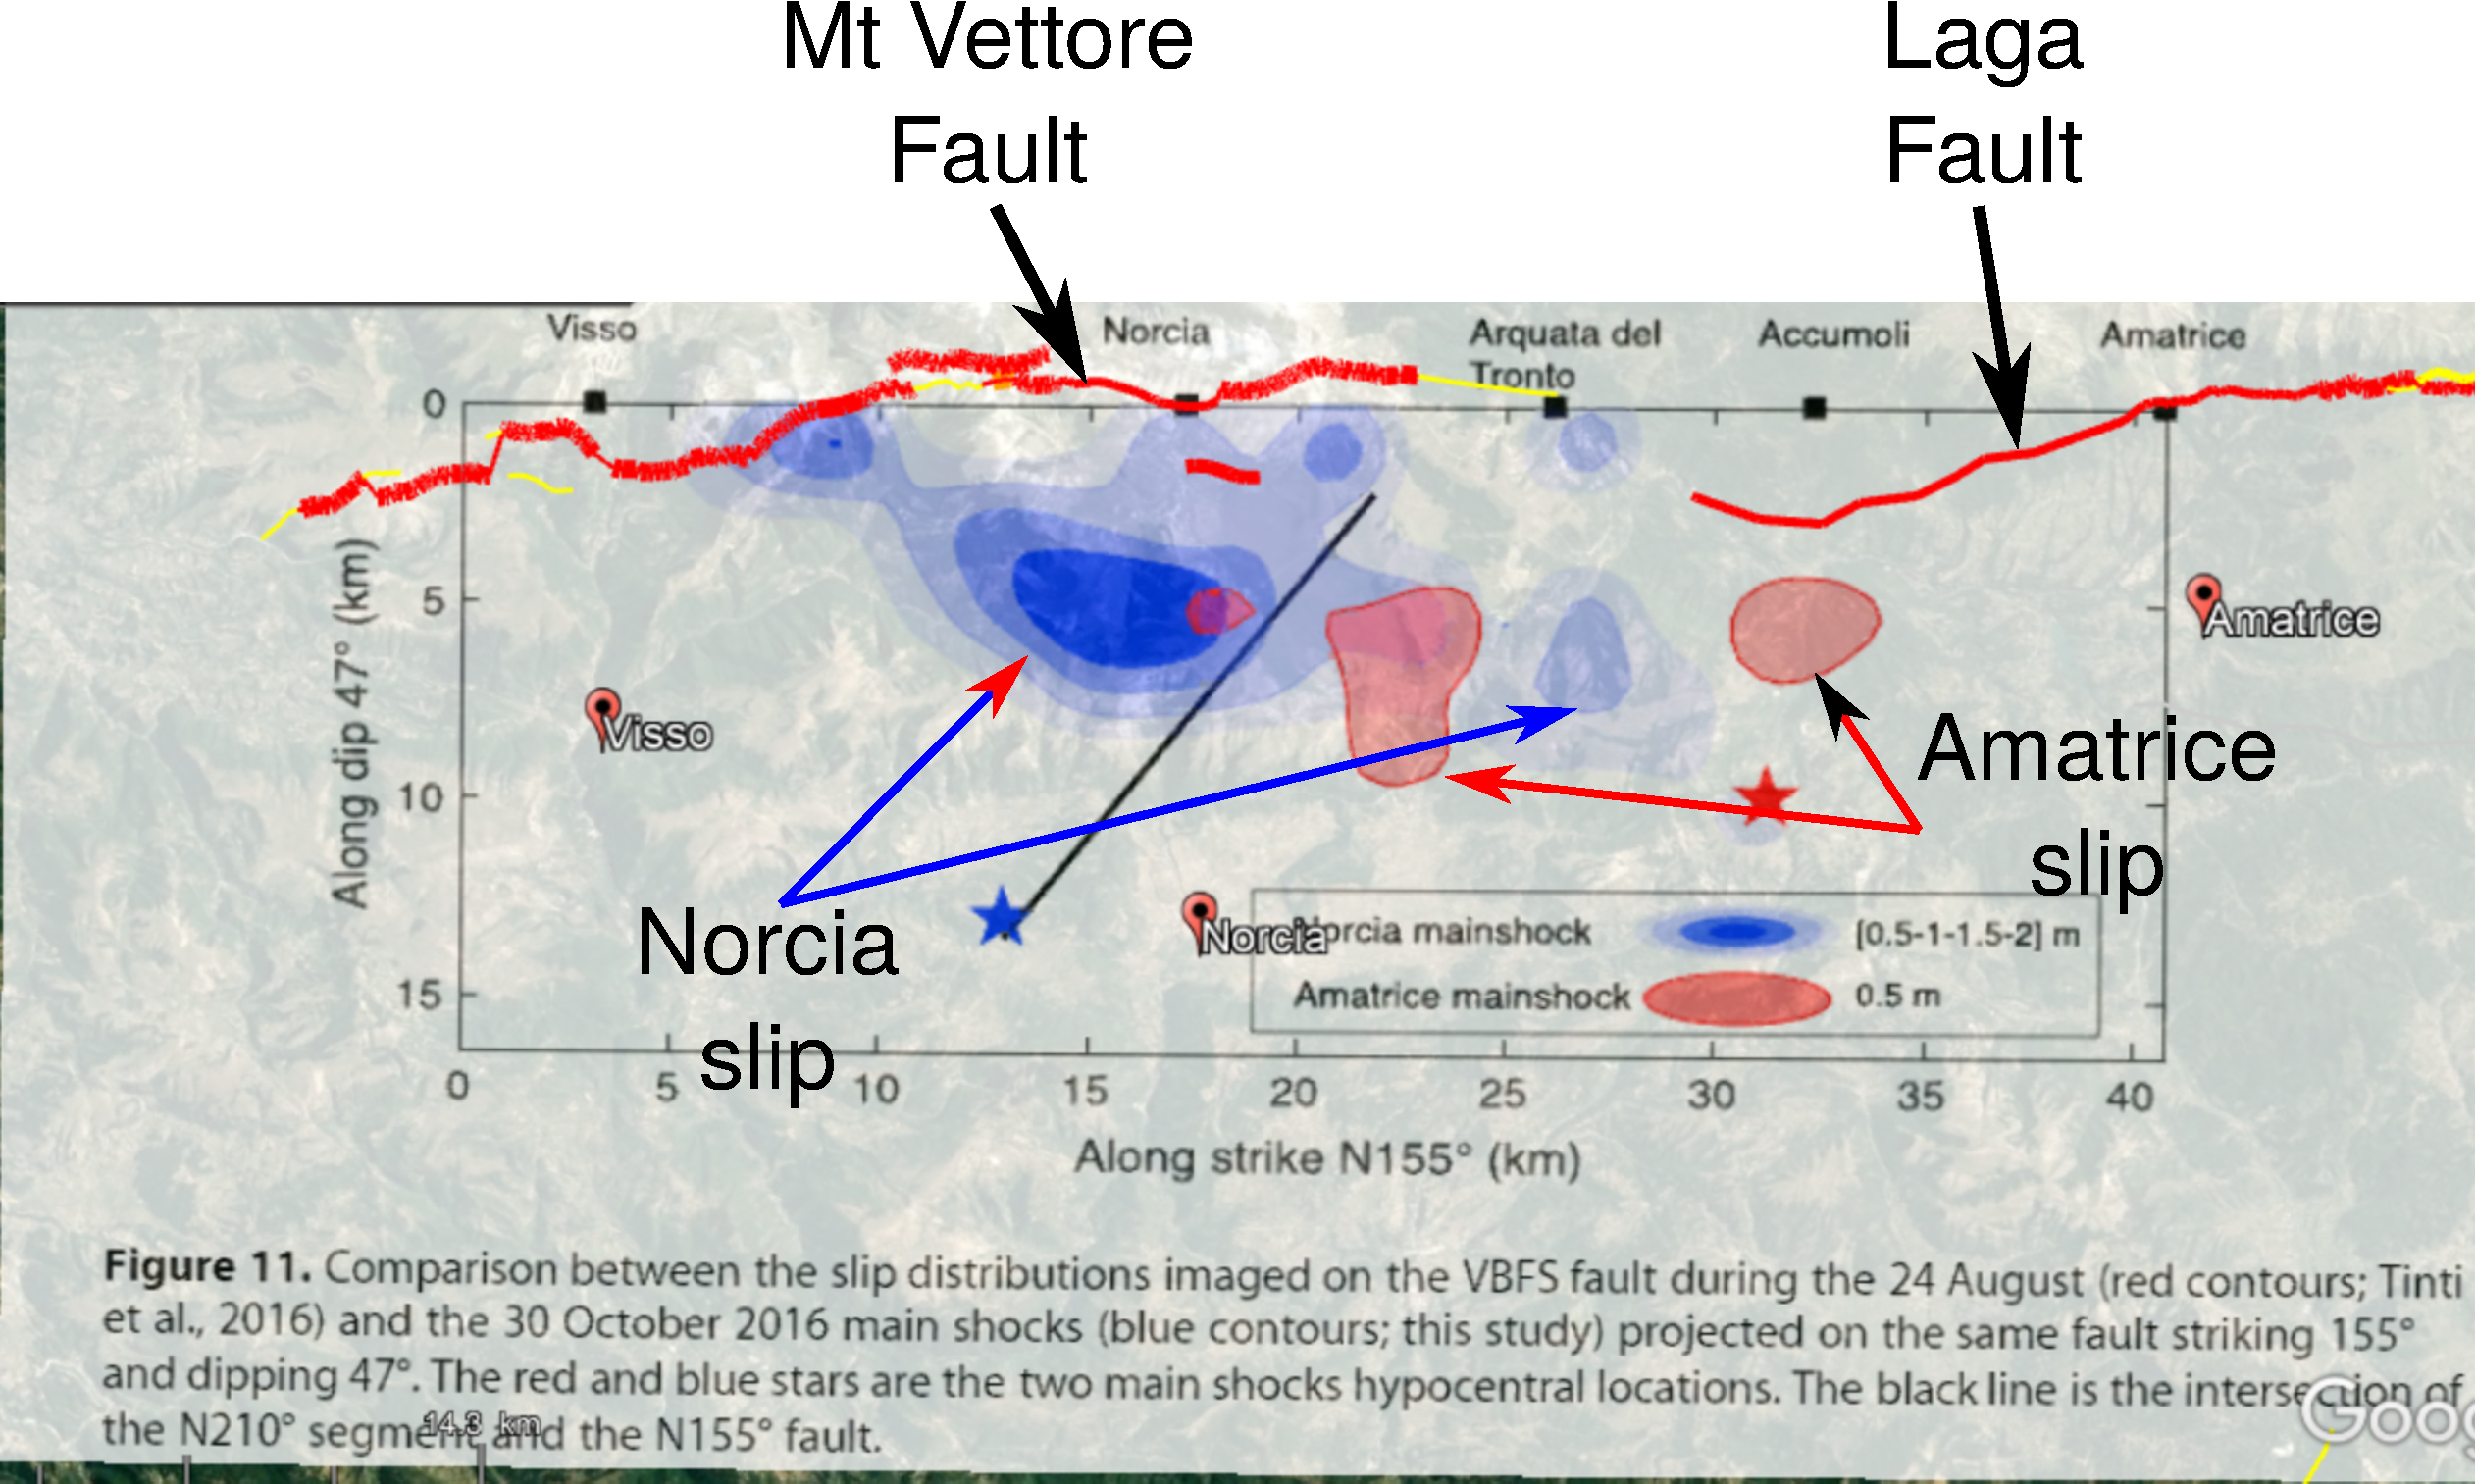
\includegraphics[width=0.65\linewidth]{images/amatrice_3.pdf} \,
  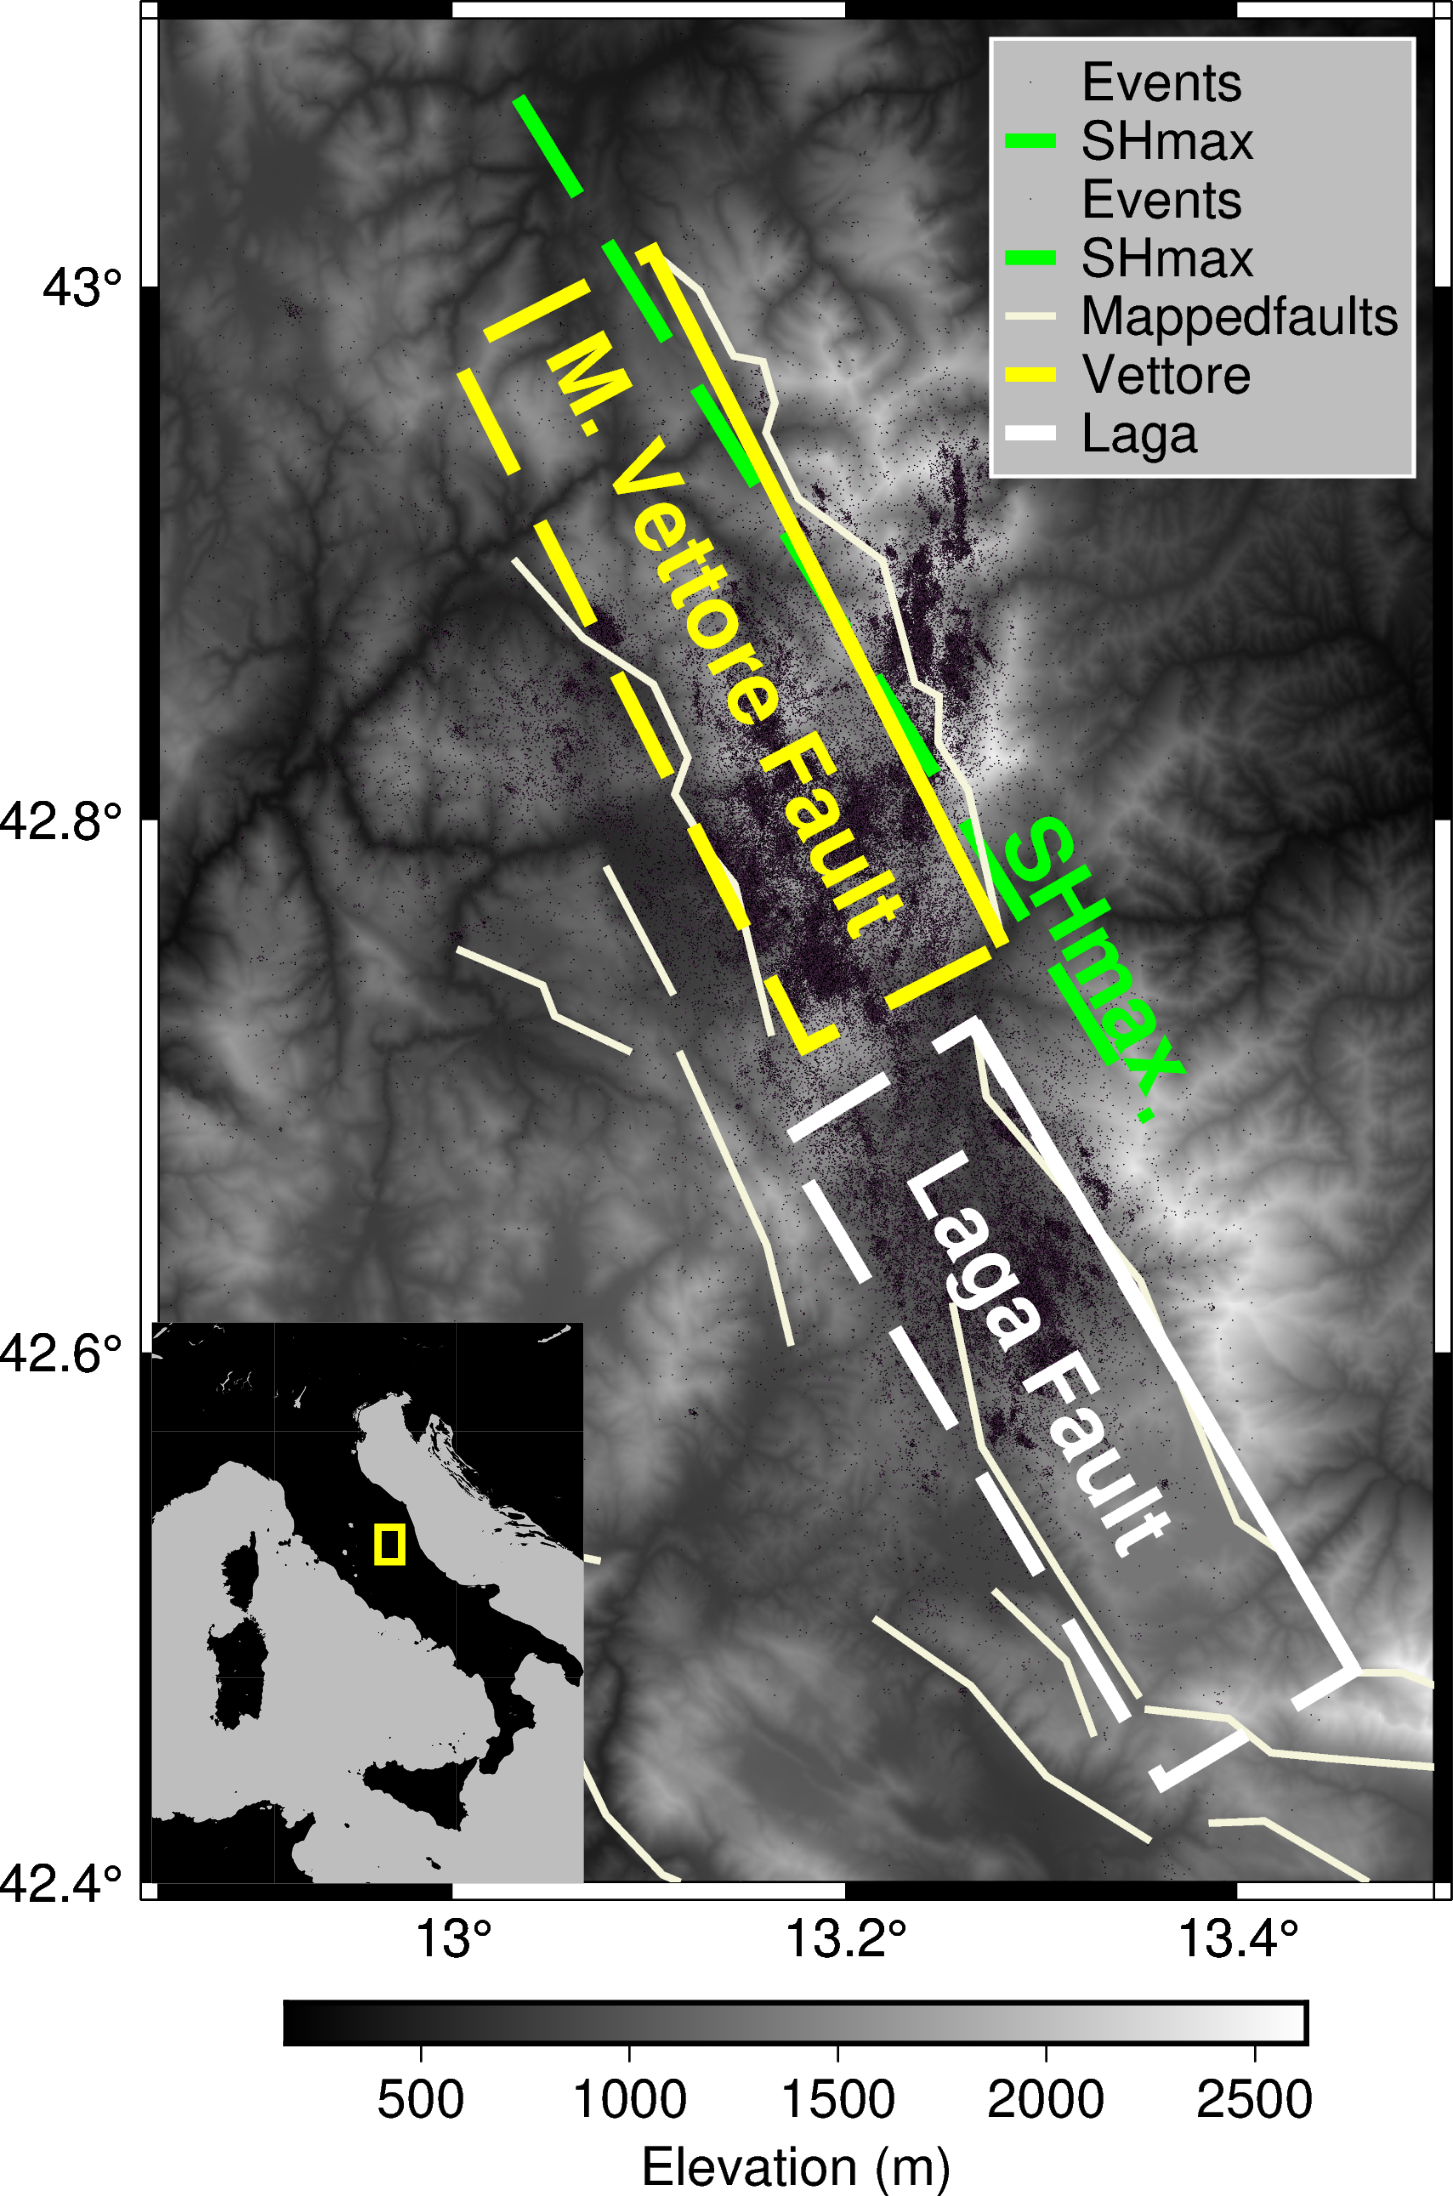
\includegraphics[width=0.3\linewidth]{images/map_italy.png}  
 \end{center}
  \vskip 0.2cm
  {\bf \hfill \scriptsize Modified by O. Scotti from \cite{Scognamiglio_2018_CFG}}
  \addtocounter{framenumber}{-1}
  
\end{frame}


\begin{frame}
 {Seismic Hazard in Central Italy}
 
 \begin{center}
  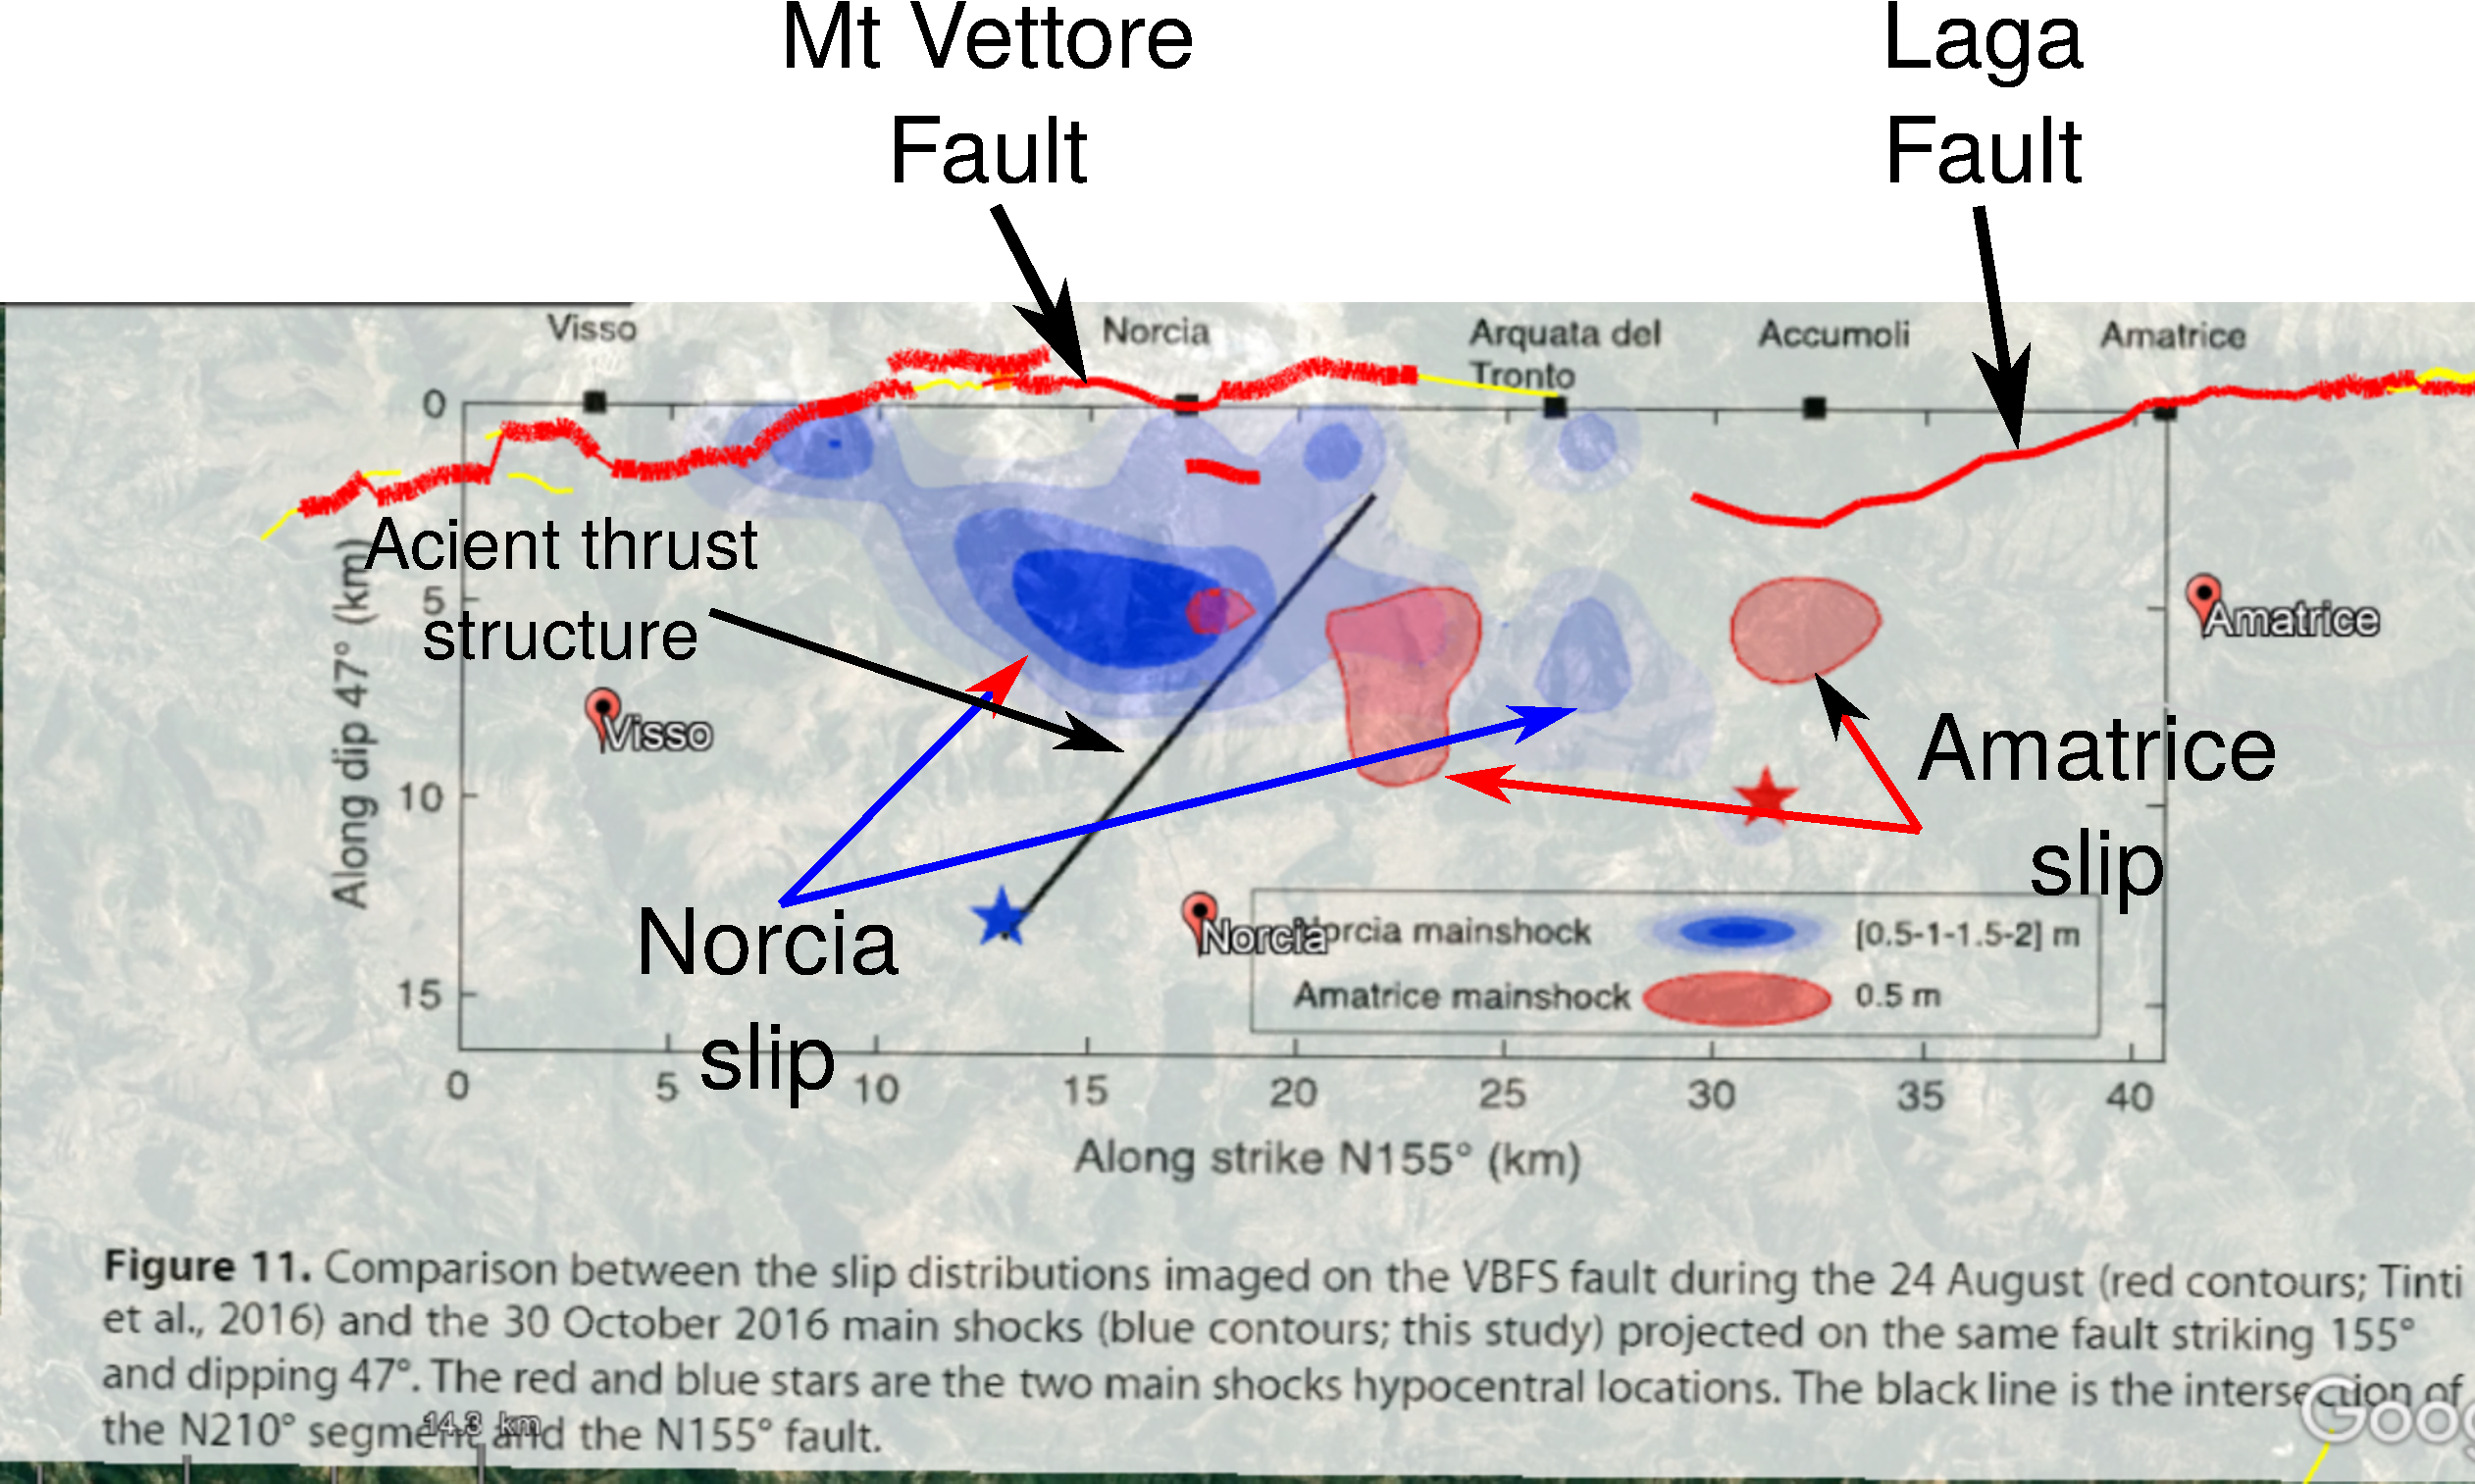
\includegraphics[width=0.65\linewidth]{images/amatrice_4.pdf} \,
  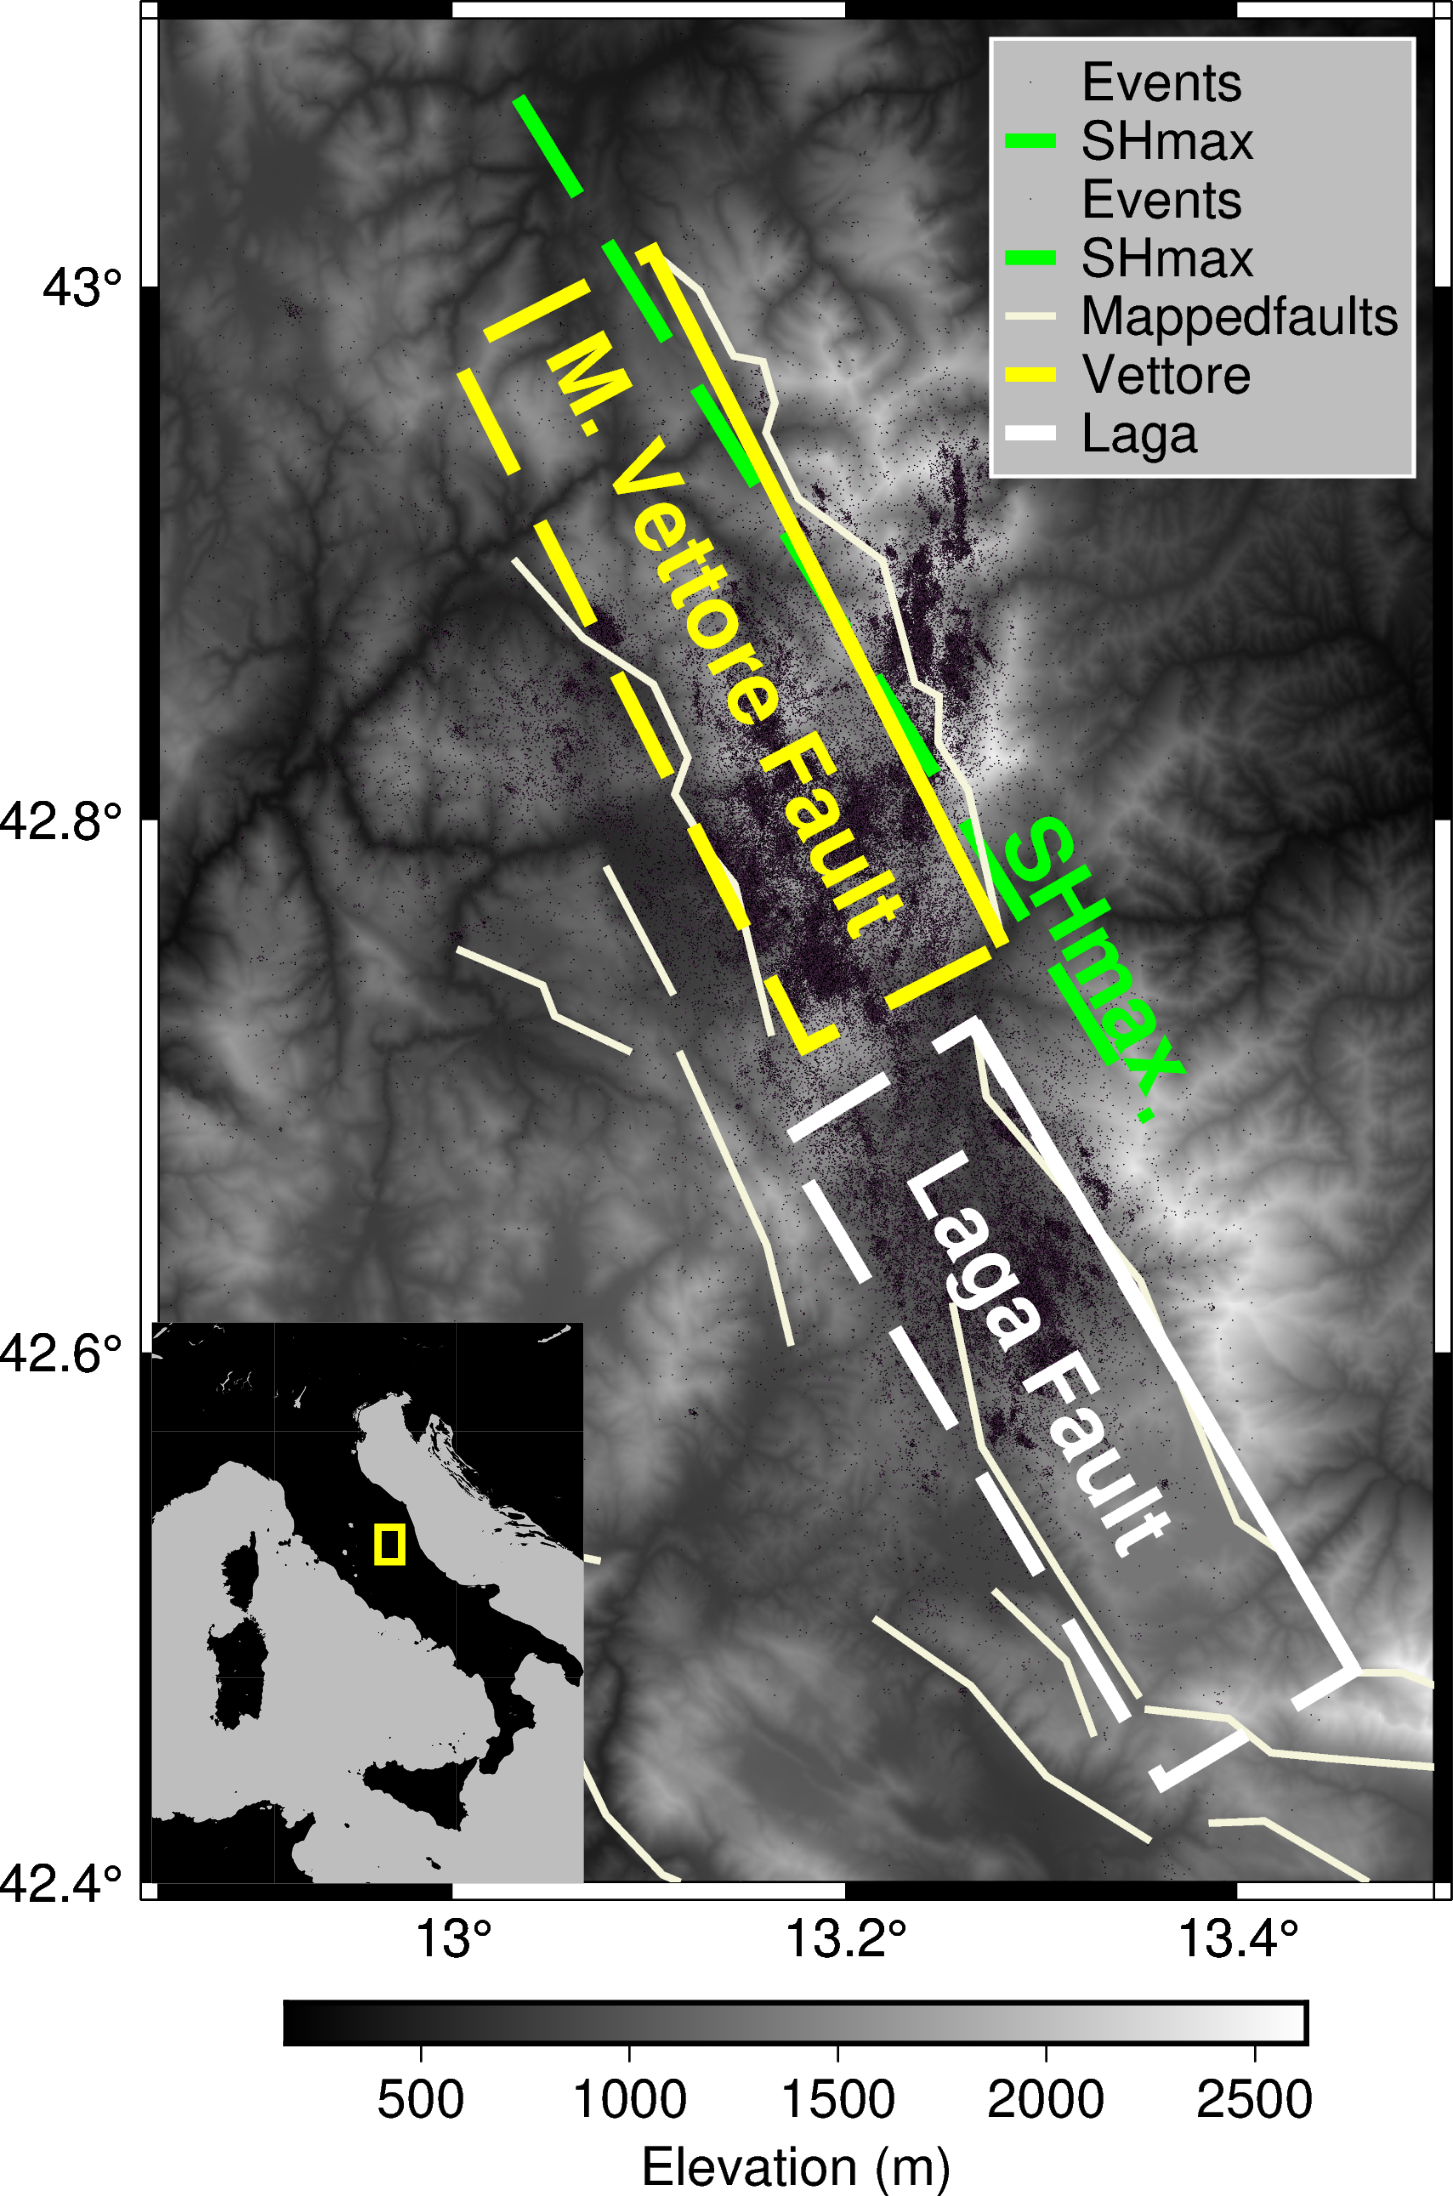
\includegraphics[width=0.3\linewidth]{images/map_italy.png}  
 \end{center}

  \vskip 0.2cm
  {\bf \hfill \scriptsize Modified by O. Scotti from \cite{Scognamiglio_2018_CFG}}
  \addtocounter{framenumber}{-1}
  
\end{frame}


\begin{frame}
 {Seismic Hazard in Central Italy}
 
 \begin{minipage}{0.45\linewidth}
  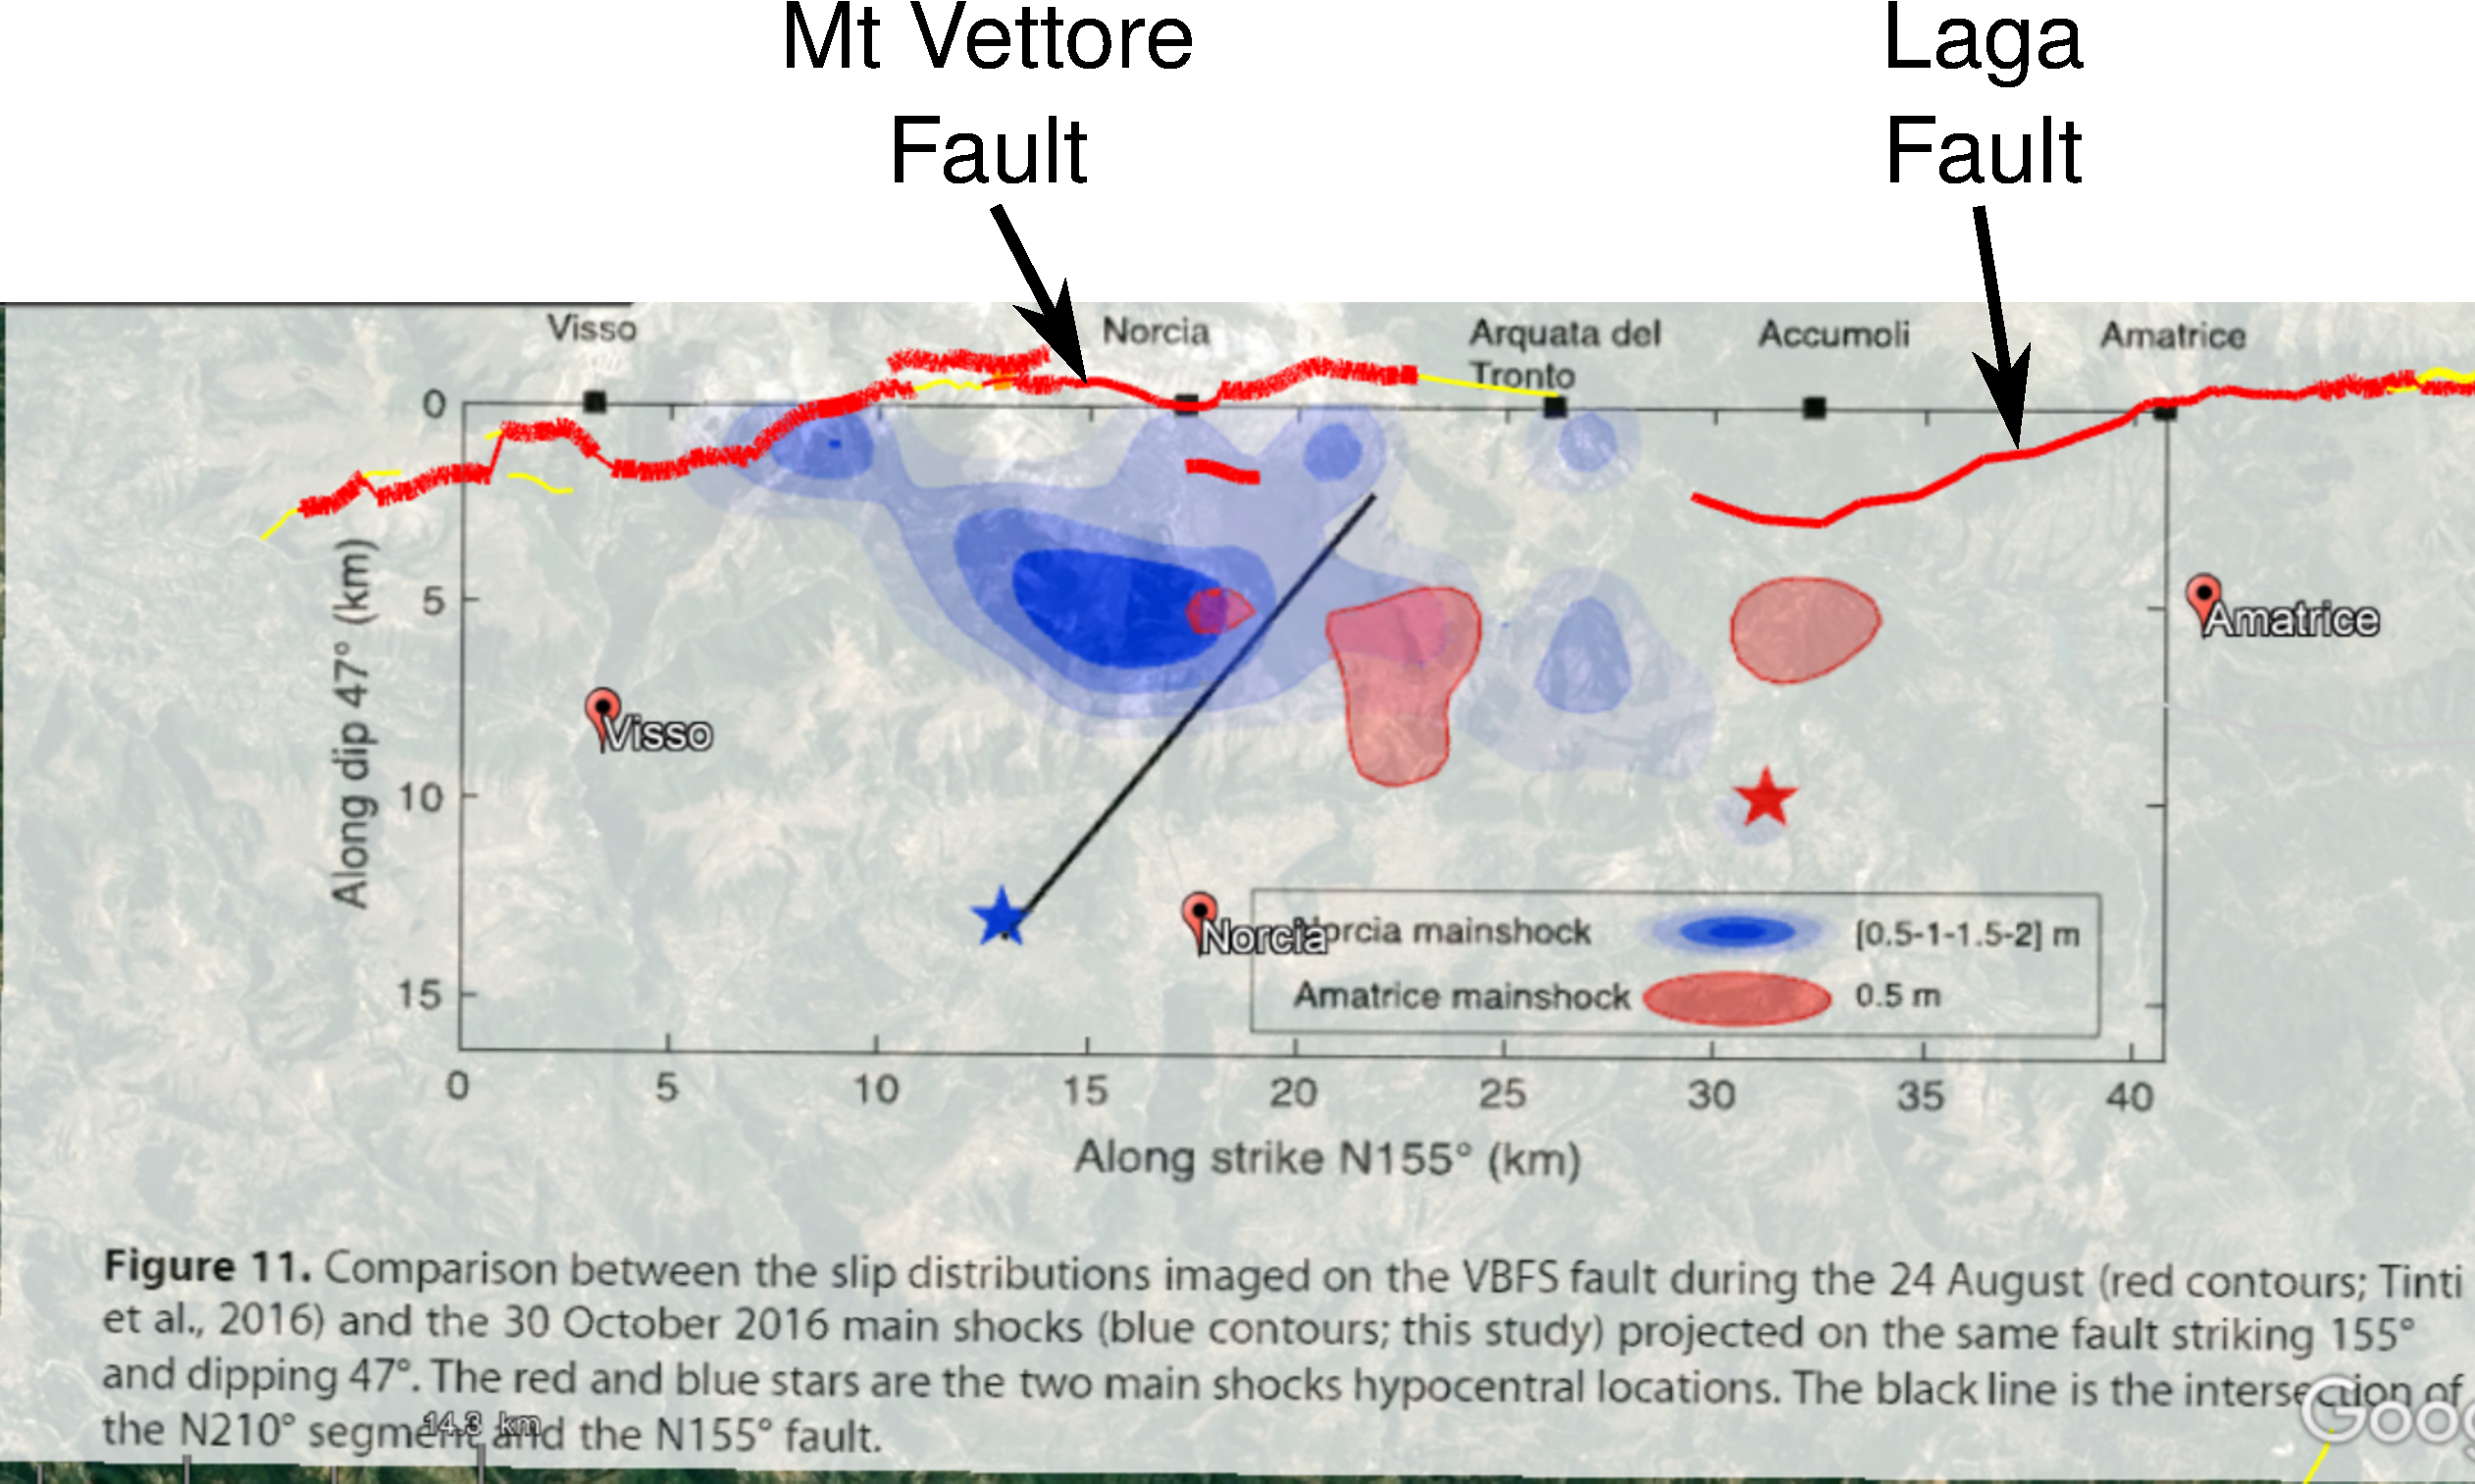
\includegraphics[width=1\linewidth]{images/amatrice_1.pdf}
 \end{minipage}
 \begin{minipage}{0.52\linewidth}
  {\bf Rupture jump across step-overs}
  \begin{itemize}
   \footnotesize \item \footnotesize Potential larger magnitudes?
   \vskip 0.3cm
   \item \footnotesize Conditions promoting this?
   \begin{itemize}
   \vskip 0.3cm
    \item \footnotesize Geometry
    \item \footnotesize Stress conditions
   \end{itemize}
   \vskip 0.3cm
   \item \footnotesize To enhance SHA!
  \end{itemize}
 \end{minipage}

 \begin{center}
 \vskip 0.3cm
   \underline{\bf \small Investigate the physical conditons}
   \underline{\bf \small promoting rupture jumps across step overs} 
   \underline{\bf \small regarding normal fault systems} 
  \vskip 0.3cm
  
 \end{center}
 {\scriptsize Previous studies focused on strike-slip fault systems: \cite{Galis_2015_ISS,Hu_2016_IEJ,Bai_2017_ESD,Li_2020_ERT,Oglesby_2008_RTJ}, and more ... } 
 \addtocounter{framenumber}{-1}
 
\end{frame}




\section{Settings}

\begin{frame}
 {Geometry and parameters explored}
 
  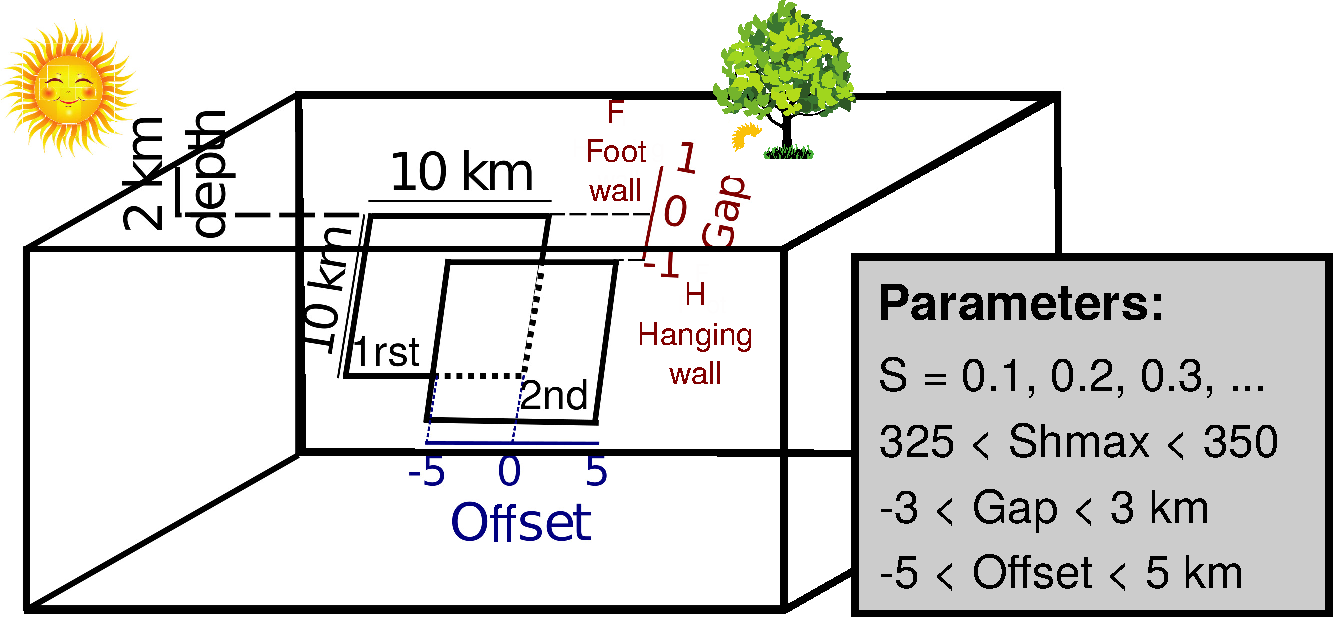
\includegraphics[width=1\linewidth]{images/schematic_view_param_new}
 
 \hfill {\tiny \citep[www.seissol.org; e.g.,][]{Wollherr_2018_OFP, Ulrich_2019_CPB}}
 
\end{frame}


\begin{frame}
 {Preliminary exploration: 3 different cases}

 \begin{center}
 For these cases: Gap = 1 km, Offset = 1 km \\
 \vskip 0.4cm
 \begin{minipage}{0.48\linewidth}
    \centering \small Only 1 fault segment breaks \\
  	\animategraphics[autoplay,loop,width=\textwidth]{1}{images/nojump/nojump_neg_00}{00}{04}
  	$S$: 0.6
 \end{minipage} \,
 \begin{minipage}{0.48\linewidth}
    \centering \small Rupture is arrested after jumping \\
  	\animategraphics[autoplay,loop,width=\textwidth]{1.2}{images/arrested/arrested_neg_00}{05}{10}
  	$S$: 0.4
 \end{minipage} \\
 \vskip 0.5cm
 \begin{minipage}{0.45\linewidth}
    \centering \small Both segments break \\
  	\animategraphics[autoplay,loop,width=\textwidth]{1}{images/jumping/jumping_neg_00}{00}{04}
  	$S$: 0.2
 \end{minipage}
 \end{center}
 \addtocounter{framenumber}{-1}
  
\end{frame}


\begin{frame}
 {Preliminary exploration: 3 different cases}

 \begin{center}
 For these cases: Gap = 1 km, Offset = 1 km \\
 \vskip 0.4cm
 \begin{minipage}{0.48\linewidth}
 \centering \small Only 1 fault segment breaks \\
  	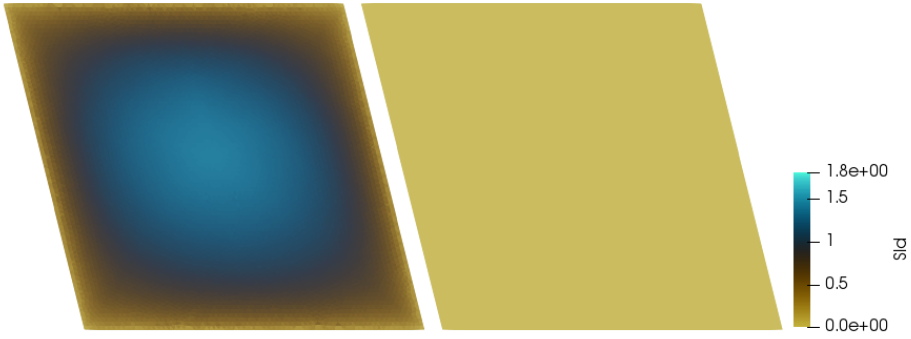
\includegraphics[width=\textwidth]{images/nojump/nojump_neg_0004.png}   
    {\bf $S$: 0.6}
 \end{minipage} \,
 \begin{minipage}{0.48\linewidth}
    \centering \small Rupture is arrested after jumping \\
  	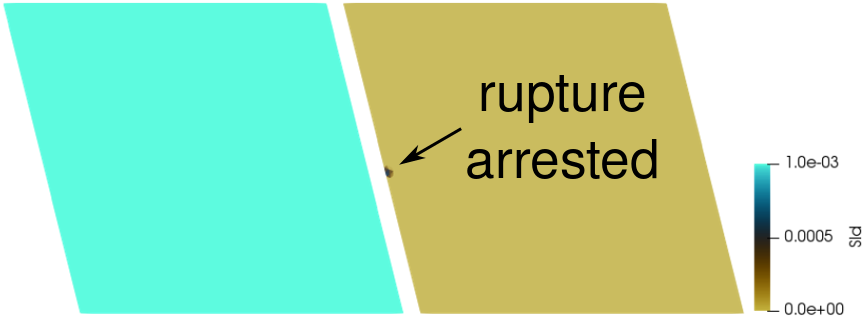
\includegraphics[width=\textwidth]{images/arrested/arrested_neg_0010.png}   
  	{\bf $S$: 0.4}
 \end{minipage} \\
 \vskip 0.5cm
 \begin{minipage}{0.45\linewidth}
    \centering \small Both segments break \\
  	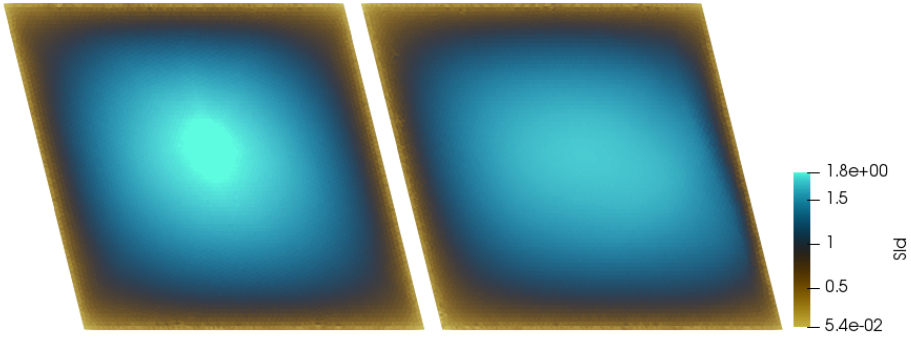
\includegraphics[width=\textwidth]{images/jumping/jumping_neg_0004.png}   
  	{\bf $S$: 0.2}
 \end{minipage}
 \end{center}
 \addtocounter{framenumber}{-1}
  
\end{frame}



\section*{References}
\begin{frame}

    {\tiny \bibliography{\dirbiblio/bibliography} }							\bibliographystyle{apalike}    

\end{frame}


\end{document}

